\hyphenation{se-para-tion}
\hyphenation{theo-re-ti-cal}
\hyphenation{handed-ness}
\hyphenation{fo-llo-wing}
\hyphenation{ac-cor-ding}

%______________________ Theory ______________________
\chapter{Theoretical approach}
\label{ch:theory}

%______________________ INTRODUCCION ______________________
\section{Introduction}
The SM uses the Lagrangian formalism to describe the interactions of elementary particles and fields. The SM Lagrangian can be split into four main terms:

\begin{itemize}
\item Gause bosons and their interactions
\item Higgs boson, its self-interaction, and interaction with the gauge bosons to give them mass, which is not possible solely by the $\Lagr_{YM}$
\item Fermions and their interactions with the gauge bosons
\item Fermions and their interactions with the Higgs boson, which through the Yukawa mechanism gives mass to fermions
\end{itemize}
 
or equivalently:
\begin{equation}\label{lagr_SM}
\Lagr_{SM} = \Lagr_{YM} + \Lagr_{H} + \Lagr_{ferm} + \Lagr_{Yuk} 
\end{equation}

The first term in the SM Lagrangian:
\beqn\label{lagr_YM}
\Lagr_{YM} = 	-\frac{1}{4}W^i_{\mu\nu}(x)W_i^{\mu\nu}(x) -\frac{1}{4}B_{\mu\nu}(x)B^{\mu\nu}(x) -\frac{1}{4}G^a_{\mu\nu}(x)G_a^{\mu\nu}(x)
\eeqn

where
\begin{align}
B_{\mu\nu}(x)   \equiv & \partial_\mu B_\nu -  \partial_\nu B_\mu \label{B_tensor} \\ 
W^i_{\mu\nu}(x) \equiv & \partial_\mu W^i_\nu(x) - \partial_\nu W^i_\mu(x) - g\varepsilon^{ijk}W^j_\mu W^k_\nu \label{W_tensor}\\
G^a_{\mu\nu}(x) \equiv & \partial_\mu G^a_\nu(x) - \partial_\nu G^a_\mu(x) - g_s f^{abc}G^b_\mu G^c_\nu \label{G_tensor}\\
\end{align}
with $i,j,k = 1,2,3$ and $a,b,c = 1, ..., 8$. The fields have the following connections to their underlying symmetries: $B_{\mu\nu}$ corresponds to $U(1)$ symmetry of the weak hypercharge $Y_k$ and "B" term is simply a kinematic term while "W" and "G" terms describe interactions among the corresponding bosons, where $W^i_{\mu\nu}$ corresponds to $SU(2)_I$ symmetry of the weak isospin $I^i_{w}$, and $G^a_{\mu\nu}$ corresponds to $SU(3)_c$ symmetry of the QCD color charge. $g$ and $\varepsilon$ are $SU(2)$ coupling and structure constants, while $g_s$ and $f$ are coupling and structure constants for $SU(3)$.

The next term in the SM Lagrangian explains how fermions interact with the gauge bosons, however, mass terms are absent:
\beqn\label{lagr_ferm}
\Lagr_{ferm}= i \bar{\Psi}_L \slashed{D} \Psi_L  + i \bar{\psi}_{l_{R}}  \slashed{D} \psi_{l_{R}} +
i \bar{\Psi}_Q \slashed{D} \Psi_Q  + i \bar{\psi}_{u_{R}}  \slashed{D} \psi_{u_{R}} +
 i \bar{\psi}_{d_{R}}  \slashed{D} \psi_{d_{R}}
\eeqn

Above $\Psi$ represents a doublet of a charged lepton and a corresponding neutral lepton within the same lepton family of $SU(2)_L$, a letter Q is reserved for a family of quarks, and $\psi_R$ describes a right-handed leptonic singlet.

\begin{align}\label{cov_der2}
D_\mu = \partial_\mu + ig I_w^i W_\mu^i+ ig' Y_w B_\mu + ig_s T_c^a G_\mu^a\\ 
\end{align}

\begin{align}\label{neutral_fields}
A_\mu = &  B_\mu \cos\theta_W + W^3_\mu \sin\theta_W \\ 
Z_\mu = & -B_\mu \sin\theta_W + W^3_\mu \cos\theta_W \nonumber 
\end{align}
\noindent where $\theta_W$ is known as the \ti{Weinberg angle}.

\noindent the Higgs Lagrangian is given by 
\beqn\label{lagr_higgs}
\Lagr_H=(D_\mu\Phi)^\dagger(D^\mu\Phi) - V(\Phi) , \qquad V(\Phi)= - \mu^2(\Phi^\dagger\Phi) + \frac{\lambda}{4}(\Phi^\dagger\Phi)^2
\eeqn

\beqn\label{lagr_Yuk}
\Lagr_{Yuk}=  - i \bar{\Psi}_{L}  G_l  \psi_{l_{R}} \Phi
- i \bar{\Psi}_{Q}  G_u  \psi_{u_{R}} \tilde{\Phi}
- i \bar{\Psi}_{Q}  G_d \psi_{d_{R}} \Phi + h.c.
\eeqn
where $\tilde{\Phi} = i \sigma^2 \Phi^*$

\beqn
\Phi = \binom{\phi^+}{\phi^0 = (v+H + i\chi)/ \sqrt{2}}
\eeqn

 
\beqn
\Phi_0^{\dagger} \Phi_0= \frac{v^2}{2}, \quad v = 2 \sqrt{\frac{\mu^2}{\lambda}}
\eeqn

\beqn
M_W = \frac{gv}{2}, \quad  M_Z = \frac{M_W}{\cos{\theta_W}}, \quad M_H = \sqrt{2\mu^2}
\eeqn


\label{secc:lagrangian}



\section{Electroweak unification and the Higgs mechanism}\label{sec:EWI}

Physicists dream of building a theory that contains all the interactions in one single interaction, \ie, showing that at some scale in energy all the four fundamental interactions are unified and only one interaction emerges in a \ti{Theory of everything}. The first sign of the feasibility of such unification came from success in the construction of the CED. Einstein spent years trying to reach that full unification, which by 1920 only involved electromagnetism and gravity, with no success; however, a new partial unification was achieved in the 1960's, when S.Glashow\cite{glashow}, A.Salam\cite{salam} and S.Weinberg \cite{weinberg} independently proposed that electromagnetic and weak interactions are two manifestations of a more general interaction called \ti{electroweak interaction (EWI)}. EWI was developed by following the useful prescription provided by QED and the gauge invariance principles.

\begin{figure}[h!]
  \centering
  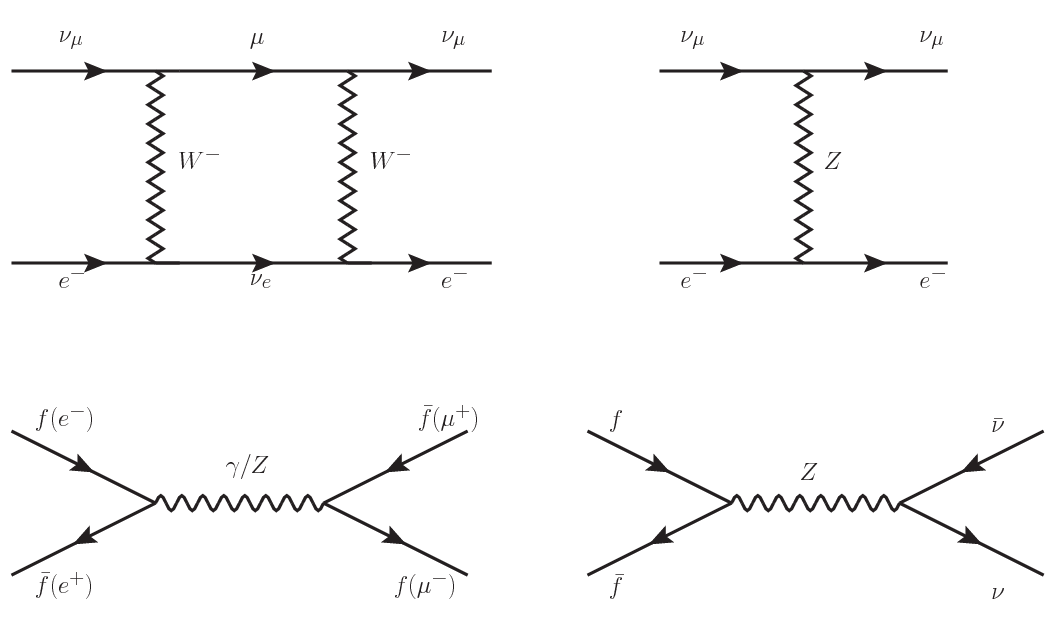
\includegraphics[scale=0.4]{nc}
  \caption[Neutral current processes]{Top: $\nu_{\mu}-e^-$ scattering going through charged currents (left) and neutral currents (right). Bottom: neutral current processes for charged fermions (left) and involving neutrinos (right). While neutral current processes involving only charged fermions can proceed through EI or WI, those involving neutrinos can only proceed via WI.}% The former can be seen as an indication that at some level WI and EI are closely connected.}
         \label{nc}
\end{figure}

The \ti{classic} weak theory developed by Fermi, did not have the concept of the W boson but instead it was treated as a point interaction with the dimensionful constant $G_F$ associated with it. It works really well at low energies very far off the W mass shell. When going up in energy, the theory of weak interactions involving the W boson is capable of explaining the $\beta$-decay and in general the processes mediated by \wpm bosons. However, there were some processes like the \ti{$\nu_\mu - e$ scattering} which would require the exchange of two W bosons (see Figure \ref{nc} top diagrams) giving rise to divergent loop integrals and then non-finite predictions. The EWI theory, by including neutral currents involving fermions via the exchange of a neutral bosons Z, overcomes those divergences and the predictions become realistic.

Neutral weak interaction vertices conserve flavor in the same way as the electromagnetic vertices do, but additionally, the Z boson can couple to neutrinos which implies that processes involving charged fermions can proceed through EI or WI but processes involving neutrinos can proceed only through WI.   

The prescription to build a gauge theory of the WI consists of proposing a free field Lagrangian density that includes the particles involved; next, by requesting invariance under global phase transformations first and generalizing to local phase transformations invariance later, the conserved currents are identified and interactions are generated by introducing gauge fields. Given that the goal is to include the EI and WI in a single theory, the group symmetry considered should be a combination of $SU(2)_L$ and $U(1)_{em}$ , however the latter cannot be used directly because the EI treats left and right-handed particles indistinctly in contrast to the former. Fortunately, the weak hypercharge, which is a combination of the weak isospin and the electric charge (Eqn. \ref{gmn}) is suitable to be used since it is conserved by the  EI and WI. Thus, the symmetry group to be considered is

\begin{equation}
G\equiv SU(2)_L\otimes U(1)_Y
\end{equation}

The following treatment applies to any of the fermion generations, but for simplicity the first generation of leptons will be considered\cite{peskin,mandl,halzen,pich}.

Given the first generation of leptons, represented by the spinors  

\begin{equation}\label{first_gen}
\psi_1 = \binom{\nu_e}{e^-}_L , \qquad \psi_2= \nu_{eR}, \qquad \psi_3= e^-_R
\end{equation}

\noindent the charged fermionic currents are given by

\beqn\label{fermion_currents}
J_\mu \equiv  J_\mu^+ = \bar{\nu}_{eL} \gamma_\mu e_L, \qquad J_\mu^\dagger \equiv J_\mu^- = \bar{e}_L \gamma_\mu \nu_{eL} 
\eeqn

\noindent and the free Lagrangian is given by

\begin{equation}\label{lo}
\Lagr_0 = \sum_{j=1}^3 i\overline{\psi}_j(x)\gamma^\mu \partial_\mu \psi_j(x),
\end{equation}

\noindent with $\gamma^\mu$ the Dirac matrices, $\overline{\psi}$ are the adjoint spinors. Mass terms are included directly in the QED free Lagrangians since they preserve the invariance under the symmetry transformations involved which treat left and right handed particles similarly, however mass terms of the form

\beqn 
m_W^2W_\mu^\dagger(x)W^\mu(x) + \frac{1}{2}m_Z^2Z_\mu(x)Z^\mu(x) -m_e\bar{\psi_e}(x)\psi_e(x).
\eeqn
\noindent which represent the mass of \wpm, Z bosons and electrons are not invariant under G transformations, therefore the gauge fields described by the EWI are in principle massless.

Experiments have shown that the EWI gauge fields are not massless\cite{wmass1,wmass2,zmass1,zmass2}; however, they have to acquire mass through a mechanism compatible with the gauge invariance; that mechanism is known as the \ti{Higgs mechanism} and will be considered later in this Section. The global transformations in the combined symmetry group G can be written as

\begin{align}\label{G_transf}
\psi_1(x) \xrightarrow[]{G}\psi'_1(x)\equiv &U_YU_L\psi_1(x),\nonumber\\ 
\psi_2(x) \xrightarrow[]{G}\psi'_2(x)\equiv &U_Y\psi_2(x),\\
\psi_3(x) \xrightarrow[]{G}\psi'_3(x)\equiv &U_Y\psi_3(x)\nonumber
\end{align}
\noindent where $U_L$ represent the $SU(2)_L$ transformation acting only on the weak isospin doublet and $U_Y$ represent the $U(1)_Y$ transformation acting on all the weak isospin multiplets. Explicitly
\beqn
U_L\equiv \exp \left(i\frac{\sigma_i}{2}\alpha^i\right), \qquad U_Y\equiv \exp(iy_i\beta) \qquad (i=1,2,3)
\eeqn
\noindent with $\sigma_i$ the Pauli matrices and $y_i$ the weak hypercharges. In order to promote the transformations from global to local while keeping the invariance, it is required that $\alpha^i=\alpha^i(x)$, $\beta=\beta(x)$ and the replacement of the ordinary derivatives by the covariant derivatives

\begin{align}\label{cov_der2}
D_\mu \psi_1(x) \equiv &\left[\partial_\mu + ig\sigma_i W_\mu^i(x)/2+ ig'y_1B_\mu(x)\right]\psi_1(x)\nonumber\\ 
D_\mu \psi_2(x) \equiv &\left[\partial_\mu + ig'y_2B_\mu(x)\right]\psi_2(x)\\
D_\mu \psi_3(x) \equiv &\left[\partial_\mu + ig'y_3B_\mu(x)\right]\psi_3(x)\nonumber 
\end{align}

\noindent introducing in this way four gauge fields, $W_\mu^i(x)$ and $B_\mu(x)$, in the process. The covariant derivatives (Eqn. \ref{cov_der2}) are required to transform in the same way as fermion fields $\psi_i(x)$ themselves, therefore, the gauge fields transform as:

\begin{align}\label{f_transf}
B_\mu(x) \xrightarrow[]{G} B_\mu'(x)\equiv & B_\mu(x)
- \frac{1}{g'}\partial_\mu\beta(x) \nonumber\\
W^i_\mu(x) \xrightarrow[]{G} W_\mu^{i\prime}(x)\equiv & W^i_\mu(x) - \frac{i}{g}\partial_\mu \alpha_i(x) - \varepsilon_{ijk}\alpha_i(x)W^i_\mu(x).
\end{align}

The G invariant version of the Lagrangian density \ref{lo} can be written as

\begin{equation}\label{linv}
\Lagr_0 = \sum_{j=1}^3 i\overline{\psi}_j(x)\gamma^\mu D_\mu \psi_j(x)
\end{equation}

\noindent where free massless fermion and gauge fields and fermion-gauge boson interactions are included. The EWI Lagrangian density must additionally include kinetic terms for the gauge fields ($\Lagr_G$) which are built from the field strengths, according to

\begin{align}
B_{\mu\nu}(x)   \equiv & \partial_\mu B_\nu -  \partial_\nu B_\mu \label{B_tensor} \\ 
W^i_{\mu\nu}(x) \equiv & \partial_\mu W^i_\nu(x) - \partial_\nu W^i_\mu(x) - g\varepsilon^{ijk}W^j_\mu W^k_\nu \label{W_tensor}
\end{align}

\noindent the last term in Eqn. \ref{W_tensor} is added in order to hold the gauge invariance; therefore,

\beqn\label{lg}
\Lagr_G = -\frac{1}{4}B_{\mu\nu}(x)B^{\mu\nu}(x)-\frac{1}{4}W^i_{\mu\nu}(x)W_i^{\mu\nu}(x)
\eeqn

\noindent which contains not only the free gauge fields contributions, but also the gauge fields self-interactions and interactions among them.

The three weak isospin conserved currents resulting from the $SU(2)_L$ symmetry are given by

\beqn
J_\mu^i(x)=\frac{1}{2}\bar{\psi_1}(x)\gamma_\mu \sigma^i \psi_1(x) 
\eeqn

\noindent while the weak hypercharge conserved current resulting from the $U(1)_Y$ symmetry is given by 

\beqn
J_\mu^Y = \sum_{j=1}^3 \overline{\psi}_j(x)\gamma_\mu y_j\psi_j(x)
\eeqn

In order to evaluate the electroweak interactions modeled by an isotriplet field $W^i_\mu$ that couples to isospin currents $J^i_\mu$ with strength $g$ and additionally the singlet field $B_\mu$ which couples to the weak hypercharge current $J_\mu^Y$ with strength $g'/2$. The interaction Lagrangian density to be considered is

\beqn
\Lagr_I = -gJ^{i\mu}(x)W_\mu^i(x)- \frac{g'}{2}J^{Y\mu}(x)B_\mu(x)
\eeqn

%\noindent written in terms of the physical fields $\wpm_\mu$, $Z_\mu$ and $A_\mu$.

Note that the weak isospin currents are not the same as the charged fermionic currents that were used to describe the WI (Eqn. \ref{fermion_currents}), since the weak isospin eigenstates are not the same as the mass eigenstates, but they are closely related

\beqn\label{fermion_currents2}
J_\mu = \frac{1}{2}(J_\mu^1 + iJ_\mu^2) ,  \qquad  J_\mu^\dagger = \frac{1}{2}(J_\mu^1 - iJ_\mu^2).
\eeqn

The same happens with the gauge fields $W^i_\mu$ which are related to the mass eigenstates \wpm by     

\beqn\label{wboson_mass_eigen}
W^+_\mu = \frac{1}{\sqrt{2}}(W_\mu^1-iW_\mu^2), \qquad W^-_\mu = \frac{1}{\sqrt{2}}(W_\mu^1+iW_\mu^2).
\eeqn

The fact that there are three weak isospin conserved currents is an indication that in addition to the charged fermionic currents, which couple charged to neutral leptons, there should be a neutral fermionic current that does not involve electric charge exchange; therefore, it couples neutral fermions or fermions of the same electric charge. The third weak isospin current contains a term that is similar to the electromagnetic current ($j_\mu^{em}$), indicating that there is a relation between them  and resembling the Gell-Mann-Nishijima formula \ref{gmn} adapted to electroweak interactions
\begin{equation}
Q=T_3 + \frac{Y_W}{2}.
\label{gmn_ew}
\end{equation}

Just as Q generates the $U(1)_{em}$ symmetry, the weak hypercharge generates the $U(1)_Y$ symmetry as said before. It is possible to write the relationship in terms of the currents as

\beqn \label{neutral_currents}
j_\mu^{em} = J_\mu^3  + \frac{1}{2}J_\mu^Y.
\eeqn

The neutral gauge fields $W^3_\mu$ and $B_\mu$ cannot be directly identified with the $Z$ and the photon fields since the photon interacts similarly with left and right-handed fermions; however, they are related through a linear combination given by

\begin{align}\label{neutral_fields}
A_\mu = &  B_\mu \cos\theta_W + W^3_\mu \sin\theta_W \\ 
Z_\mu = & -B_\mu \sin\theta_W + W^3_\mu \cos\theta_W \nonumber 
\end{align}

\noindent where $\theta_W$ is known as the \ti{Weinberg angle.} The interaction Lagrangian is now given by

\begin{align}
\Lagr_I =-\frac{g}{\sqrt{2}}(J^\mu W_\mu^+ + J^{\mu\dagger}W_\mu^-) -\left(g\sin\theta_W J_\mu^3 + g'\cos\theta_W \frac{J_\mu^Y}{2} \right)A^\mu \\ \nonumber
- \left(g\cos\theta_W J_\mu^3 - g'\sin\theta_W \frac{J_\mu^Y}{2} \right)Z^\mu 
\end{align}

\noindent the first term is the weak charged current interaction, while the second term is the electromagnetic interaction under the condition
\beqn
g\sin\theta_W = g'\cos\theta_W = e, \quad \frac{g'}{g}= \tan\theta_W  
\eeqn
\noindent contained in the Eqn.\ref{neutral_currents}; the third term is the neutral weak current.

Note that the neutral fields transformation given by the Eqn. \ref{neutral_fields} can be written in terms of the coupling constants $g$ and $g'$ as:
\beqn\label{neutral_bosons}
A_\mu= \frac{g'W_\mu^3 + gB_\mu}{\sqrt{g^2+g'^2}}, \qquad  Z_\mu= \frac{gW_\mu^3 - g'B_\mu}{\sqrt{g^2+g'^2}}.
\eeqn

So far, the Lagrangian density describing the non-massive EWI is:
\beqn\label{nmewi_lagr}
\Lagr_{nmEWI}=\Lagr_0 +\Lagr_G
\eeqn
\noindent where fermion and gauge fields have been considered massless because their regular mass terms are manifestly non invariant under G transformations; therefore, masses have to be generated in a gauge invariant way. The mechanism by which this goal is achieved is known as the \ti{Higgs mechanism} and is closely connected to the concept of \ti{spontaneous symmetry breaking.}

\subsection{Spontaneous symmetry breaking (SSB)}

Figure \ref{ssb} left shows a steel nail (top) which is subject to an external force; the form of the potential energy is also shown (bottom).

\begin{figure}[!h]
\centering
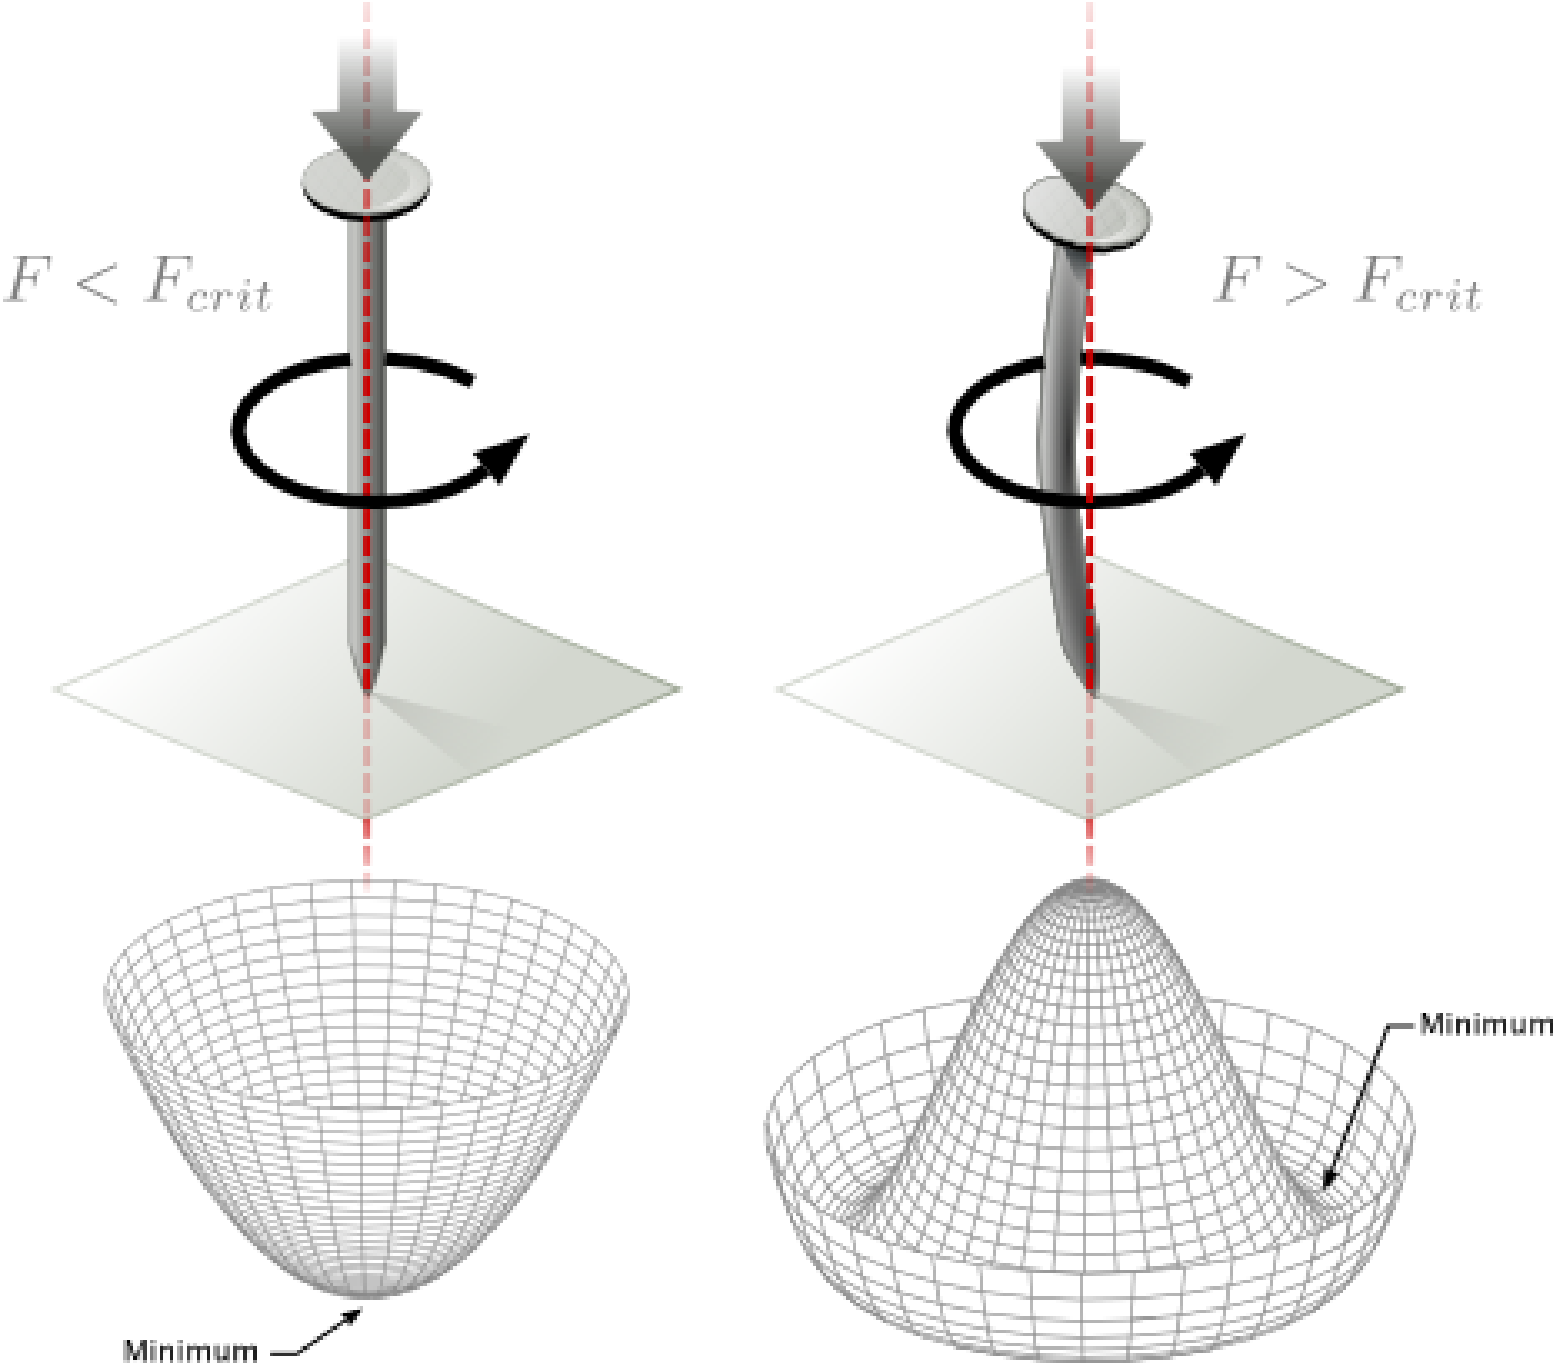
\includegraphics[scale=0.4]{broken_symmetry}
\caption[Spontaneous symmetry breaking mechanism]{Spontaneous symmetry breaking mechanism. The steel nail, subject to an external force (top left), has rotational symmetry with respect to its axis. When the external force overcomes a critical value the nail buckles (top right) choosing a minimal energy state (ground state) and thus \textit{breaking spontaneously the rotational symmetry}. The potential energy (bottom) changes but holds the rotational symmetry; however, an infinite number of asymmetric ground states are generated and circularly distributed in the bottom of the potential\cite{broken_symmetry}.}
\label{ssb}
\end{figure}

Before reaching the critical force value, the system has rotational symmetry with respect to the nail axis; however, after the critical force value is reached the nail buckles (top right). The form of the potential energy changes from a potential with only one minimum (bottom left) to a potential with an infinite set of minima (bottom right) but preserving its rotational symmetry. Right before the nail buckles there is no indication of the direction the nail will bend because any of the directions are equivalent, but once the nail bends, choosing a direction, an arbitrary minimal energy state (ground state) is selected and it does not share the system's rotational symmetry. This mechanism for reaching an asymmetric ground state is known as \textit{spontaneous symmetry breaking}.       

The lesson from this analysis is that the way to introduce the SSB mechanism into a system is by adding the appropriate potential to it.

Figure \ref{hp2d} shows a plot of the potential $V(\phi)$ in the case of a scalar field $\phi$

\beqn\label{Higgs_potential}
V(\phi)=\mu^2\phi^\dagger\phi + \lambda(\phi^\dagger\phi)^2
\eeqn

If $\mu^2>0$ the potential has only one minimum at $\phi=0$ and describes a scalar field with mass $\mu$. If $\mu^2<0$ the potential has a local maximum at $\phi=0$ and two minima at $\phi=\pm \sqrt{-\mu^2/\lambda}$ which enables the SSB mechanism to work.

\begin{figure}[!h]
\centering
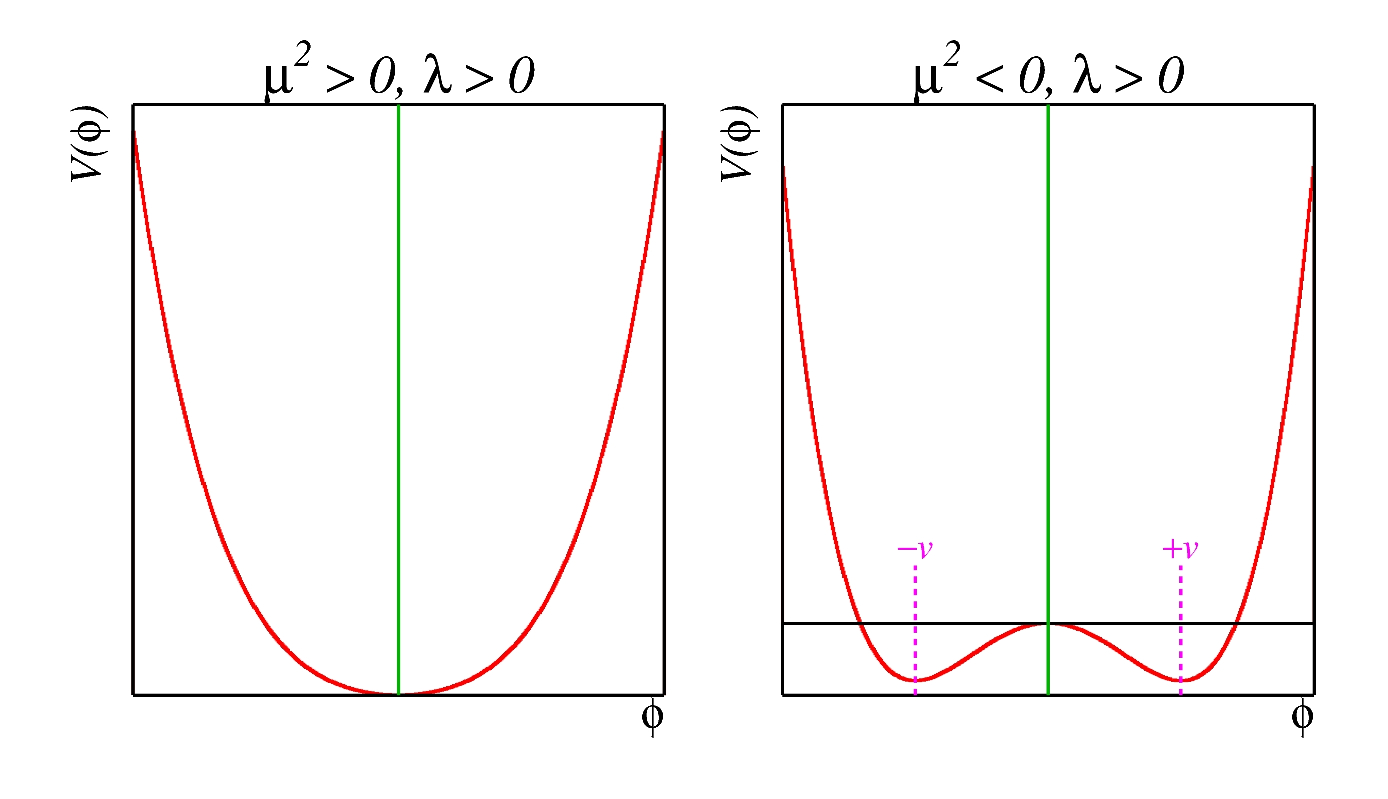
\includegraphics[width=0.6\textwidth]{hp2d}
\caption[SSB Potential form]{Shape of the potential $V(\phi)$ for $\lambda>0$ and: $\mu^2>0$ (left) and $\mu^2<0$ (right). The case $\mu^2<0$ corresponds to the potential suitable for introducing the SSB mechanism by choosing one of the two ground states which are connected via reflection symmetry. \cite{broken_symmetry}.}
\label{hp2d}
\end{figure}

In the case of a complex scalar field $\phi(x)$

\beqn\label{complex_scalar}
\phi(x)=\frac{1}{\sqrt{2}}(\phi_1 + i \phi_2)
\eeqn
\noindent the Lagrangian (invariant under global $U(1)$ transformations) is given by 
\beqn\label{higgs_potential}
\Lagr=(\partial_\mu\phi)^\dagger(\partial^\mu\phi) - V(\phi) , \qquad V(\phi)=\mu^2\phi^\dagger\phi + \lambda(\phi^\dagger\phi)^2
\eeqn

\noindent where an appropriate potential has been added in order to introduce the SSB.

As seen in Figure \ref{higgs_potential_plot}, the potential has now an infinite number of minima circularly distributed along the $\xi$-direction which makes possible the occurrence of the SSB by choosing an arbitrary ground state; for instance, $\xi=0$, \ie $\phi_1=v, \phi_2=0$

\begin{figure}[!h]
\centering
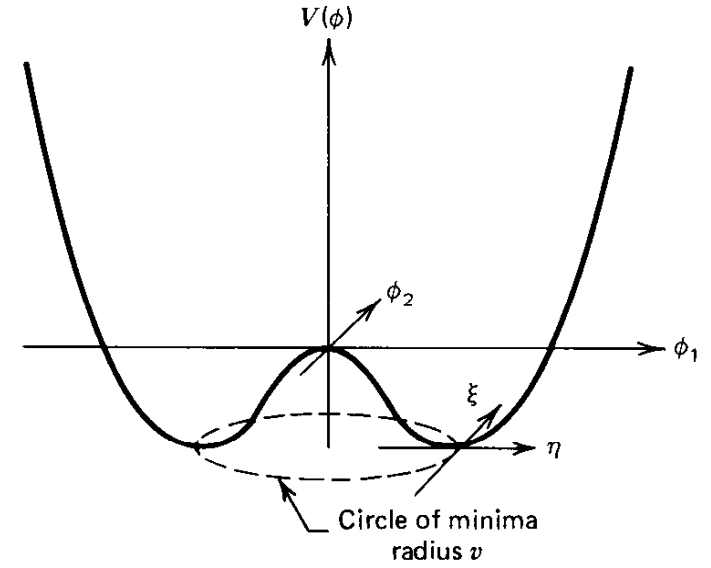
\includegraphics[scale=0.3]{higgs_potential_plot}
\caption[Potential for complex scalar field ]{Potential for complex scalar field. There is a circle of minima of radius \textit{v} along the $\xi$-direction\cite{halzen}.}
\label{higgs_potential_plot}
\end{figure}

\beqn
\phi_0=\frac{v}{\sqrt{2}}\exp(i\xi) \quad \xrightarrow[]{SSB} \quad \phi_0=\frac{v}{\sqrt{2}}
\eeqn

As usual, excitations over the ground state are studied by making an expansion about it; thus, the excitations can be parametrized as:
\beqn
\phi(x)=\frac{1}{\sqrt{2}}(v + \eta(x) + i\xi(x))
\eeqn

\noindent which when substituted into Eqn. \ref{higgs_potential} produces a Lagrangian in terms of the new fields $\eta$ and $\xi$

\beqn\label{lagr_complex_field}
\Lagr'=\frac{1}{2}(\partial_\mu\xi)^2 + \frac{1}{2}(\partial_\mu\eta)^2 + \mu^2\eta^2 - V(\phi_0) - \lambda v \eta(\eta^2+\xi^2) -  \frac{\lambda}{4}(\eta^2+\xi^2)^2
\eeqn

\noindent where the last two terms represent the interactions and self-interaction between the two fields $\eta$ and $\xi$. The particular feature of the SSB mechanism is revealed when looking to the first three  terms of $\Lagr'$. Before the SSB, only the massless $\phi$ field is present in the system; after the SSB there are two fields of which the $\eta$-field has acquired mass $m_\eta=\sqrt{-2\mu^2}$ while the $\xi$-field is still massless (see Figure \ref{higgs_hat}). 

\begin{figure}[!h]
\centering
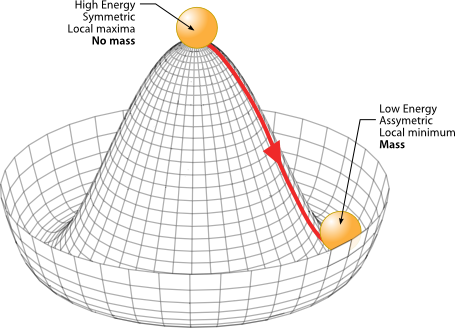
\includegraphics[width=0.48\textwidth]{higgs_hat}
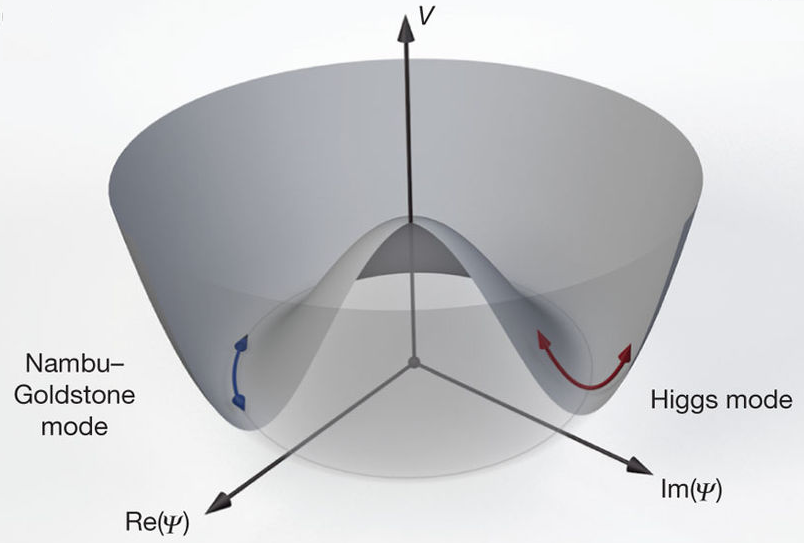
\includegraphics[width=0.5\textwidth]{goldstone_boson_mode}
\caption[SSB mechanism for complex scalar field]{SSB mechanism for a complex scalar field\cite{broken_symmetry,endres}.}
\label{higgs_hat}
\end{figure}

Thus, \textit {the SSB mechanism serves as a method to generate mass but as a side effect a massless field is introduced in the system}. This fact is known as the Goldstone theorem and states that a massless scalar field appears in the system for each continuous symmetry spontaneously broken. Another version of the Goldstone theorem states that \textit{``if a Lagrangian is invariant under a continuous symmetry group G, but the vacuum is only invariant under a subgroup $H\subset G$, then there must exist as many massless spin-0 particles (Nambu-Goldstone bosons) as broken generators.''}\cite{pich} The Nambu-Goldstone boson can be understood considering that the potential in the ${\xi-\textrm{direction}}$ is flat so excitations in that direction are not energy consuming and thus represent a massless state.                   

\subsection{Higgs mechanism}

When the SSB mechanism is introduced in the formulation of the EWI in an attempt to generate the mass of the so far massless gauge bosons and fermions, an interesting effect is revealed.

In order to keep the G symmetry group invariance and generate the mass of the EW gauge bosons, a G invariant Lagrangian density ($\Lagr_S$) has to be added to the non massive EWI Lagrangian (Eqn. \ref{nmewi_lagr})

\begin{align}
\Lagr_S    = &(D_\mu\phi)^\dagger(D^\mu\phi) - \mu^2\phi^\dagger\phi - \lambda(\phi^\dagger\phi)^2 , \qquad \lambda>0, \mu^2<0 \label{ls}\\
D_\mu\phi = &\left(i\partial_\mu - g\frac{\sigma_i}{2}W^i_\mu -
g'\frac{Y}{2}B_\mu\right)\phi
\end{align}

\noindent $\phi$ has to be an isospin doublet of complex scalar fields so it preserves the G invariance; thus $\phi$ can be defined as:

\beqn
\phi = \binom{\phi^+}{\phi^0} \equiv \frac{1}{\sqrt{2}}\binom{\phi_1 + i\phi_2}{\phi_3 + i\phi_4}.
\eeqn

The minima of the potential are defined by

\beqn
\phi^\dagger\phi=\frac{1}{2}(\phi_1^2 +\phi_2^2 +\phi_3^2 + \phi_1^4 )= -\frac{\mu^2}{2\lambda}.
\eeqn

The choice of the ground state is critical. By choosing a ground state, invariant under $U(1)_{em}$ gauge symmetry, the photon will remain massless and the $\wpm$ and $Z$ bosons masses will be generated which is exactly what is needed. In that sense, the best choice corresponds to a weak isospin doublet with $T_3=-1/2$, $Y_W=1$ and $Q=0$ which defines a ground state with $\phi_1=\phi_2=\phi_4$ and $\phi_3=v$:

\beqn\label{field_exp}
\phi_0\equiv\frac{1}{\sqrt{2}}\binom{0}{v}, \qquad v^2\equiv-\frac{\mu^2}{\lambda}.
\eeqn

\noindent where the vacuum expectation value $v$ is fixed by the Fermi coupling $G_F$ according to $v=(\sqrt{2}G_F)^{1/2}\approx 246$ GeV.

The G symmetry has been broken and three Nambu-Goldstone bosons will appear. The next step is to expand $\phi$ about the chosen ground state as:
\beqn
\phi(x) = \frac{1}{\sqrt{2}}\exp\left(\frac{i}{v}\sigma_i\theta^i(x)\right) \binom{0}{v+H(x)}\approx \frac{1}{\sqrt{2}}\binom{\theta_1(x) + i\theta_2(x)}{v + H(x) - i\theta_3(x)} 
\eeqn

\noindent to describe fluctuations from the ground state $\phi_0$. The fields $\theta_i(x)$ represent the Nambu-Goldstone bosons while $H(x)$ is known as \ti{Higgs field.} The fundamental feature of the parametrization used is that the dependence on the $\theta_i(x)$ fields is factored out in a global phase that can be eliminated by taking the physical \ti{unitary gauge} $\theta_i(x)=0$. Therefore the expansion about the ground state is given by:
\beqn\label{higgs_dublet}
\phi(x)\frac{1}{\sqrt{2}}\binom{0}{v+H(x)}
\eeqn

\noindent which when substituted into $\Lagr_S$ (Eqn. \ref{ls}) results in a Lagrangian containing the now massive three gauge bosons $\wpm, Z$, one massless gauge boson (photon) and the new Higgs field (H). The three degrees of freedom corresponding to the Nambu-Goldstone bosons are now integrated into the massive gauge bosons as their longitudinal polarizations which were not available when they were massless particles. The effect by which vector boson fields acquire mass after an spontaneous symmetry breaking, but without an explicit gauge invariance breaking is known as the \textit{Higgs mechanism}.

The mechanism was proposed by three independent groups: F.Englert and R.Brout in August 1964 \cite{englert}, P.Higgs in October 1964 \cite{higgs} and G.Guralnik, C.Hagen and T.Kibble in November 1964\cite{ghk}; however, its importance was not realized until S.Glashow\cite{glashow}, A.Salam\cite{salam} and S.Weinberg \cite{weinberg}, independently, proposed that electromagnetic and weak interactions are two manifestations of a more general interaction called \ti{electroweak interaction} in 1967.

\subsection{Masses of the gauge bosons}

The masses of the gauge bosons are extracted by evaluating the kinetic part of Lagrangian $\Lagr_S$ in the ground state (known also as the vacuum expectation value), \ie,

\beqn\label{gauge_masses}
\small
\left|\left(\partial_\mu - ig\frac{\sigma_i}{2}W^i_\mu -i\frac{g'}{2}B_\mu\right)\phi_0\right |^2= \left(\frac{1}{2}vg\right)^2W_\mu^+W^{-\mu} + \frac{1}{8}v^2(W_\mu^3,B_\mu)\binom{g^2 \quad -gg'}{-gg' \quad g'^2}\binom{W^{3\mu}}{B^\mu}
\eeqn

\noindent comparing with the typical mass term for a charged boson $M_W^2 W^+W^-$
\beqn
M_W=\frac{1}{2}vg.
\eeqn
The second term in the right side of the Eqn.\ref{gauge_masses} comprises the masses of the neutral bosons, but it needs to be written in terms of the gauge fields $Z_\mu$ and $A_\mu$ in order to be compared to the typical mass terms for neutral bosons, therefore using Eqn. \ref{neutral_bosons}
\begin{align}
\frac{1}{8}v^2[g^2(W_\mu^3)^2-2gg'W_\mu^3B^\mu + g'^2B_\mu^2]=&\frac{1}{8}v^2[ g W^3_\mu - g'B_\mu]^2 + 0[g'W^3_\mu + gB_\mu]^2\\
                                                             =&\frac{1}{8}v^2[\sqrt{g^2+g'^2}Z_\mu]^2 + 0[\sqrt{g^2+g'^2}A_\mu]^2\nonumber                                                             
\end{align}

\noindent and then

\beqn
M_Z= \frac{1}{2}v\sqrt{g^2+g'^2}, \qquad M_A=0 
\eeqn

\subsection{Masses of the fermions}
The lepton mass terms can be generated by introducing a gauge invariant Lagrangian term describing the Yukawa coupling between the lepton field and the Higgs field
\beqn\label{lyl}
\Lagr_{Yl}=-G_l\left[(\bar{\nu_l}, \bar{l})_L\binom{\phi^+}{\phi^0}l_R + \bar{l}_R(\phi^-,\bar{\phi}^0)\binom{\nu_l}{l}_L\right], \qquad l=e,\mu,\tau.
\eeqn

 After the SSB and replacing the usual field expansion about the ground state (Eqn.\ref{field_exp}) into $\Lagr_{Yl}$, the mass term arises
\beqn\label{lyl2}
\Lagr_{Yl}=-m_l(\bar{l}_Ll_R + \bar{l}_R{l}_L) -\frac{m_l}{v}(\bar{l}_Ll_R + \bar{l}_R{l}_L)H= -m_l \bar{l}l\left(1+ \frac{H}{v}\right)                   
\eeqn
\beqn
m_l=\frac{G_l}{\sqrt{2}}v
\eeqn
\noindent where the additional term represents the lepton-Higgs interaction. The quark masses are generated in a similar way as lepton masses but for the upper member of the quark doublet a different Higgs doublet is needed:
\beqn
\phi_c=-i\sigma_2\phi* = \binom{-\bar{\phi}^0}{\phi^-}.
\eeqn

Additionally, given that the quark isospin doublets are not constructed in terms of the mass eigenstates but in terms of the flavor eigenstates, as shown in Table\ref{T3Y}, the coupling parameters will be related to the CKM matrix elements; thus, the quark Lagrangian is given by:   

\beqn\label{lyq}
\Lagr_{Yq}=-G_d^{i,j}(\bar{u_i},\bar{d'_i})_L\binom{\phi^+}{\phi^0}d_{jR} - G_u^{i,j}(\bar{u_i},\bar{d'_i})_L\binom{-\bar{\phi^0}}{\phi^-}u_{jR} + h.c. 
\eeqn

\noindent with i,j=1,2,3. After SSB and expansion about the ground state, the diagonal form of $\Lagr_{Yq}$ is:
\beqn\label{lyq2}
\Lagr_{Yq}=-m_d^i\bar{d_i}d_i\left(1 +\frac{H}{v}\right) - m_u^i\bar{u_i}u_i\left(1 +\frac{H}{v}\right)
\eeqn

Fermion masses depend on arbitrary couplings $G_l$ and $G_{u,d}$ and are not predicted by the theory.  

\subsection{The Higgs field}

After the characterization of the fermions and gauge bosons as well as their interactions, it is necessary to characterize the Higgs field itself. The Lagrangian $\Lagr_S$ in Eqn. \ref{ls} written in terms of the gauge bosons is given by
\beqn
\Lagr_S= \frac{1}{4}\lambda v^4 + \Lagr_H +\Lagr_{HV}
\eeqn
\beqn\label{lh}
\Lagr_H= \frac{1}{2}\partial_\mu H\partial^\mu H -  \frac{1}{2}m_H^2 H^2 - \frac{1}{2v}m_H^2 H^3 -  \frac{1}{8v^2}m_H^2 H^4
\eeqn
\beqn\label{lhV}
\Lagr_{HV}= m_H^2W_\mu^+W^{\mu-}\left(1+ \frac{2}{v}H +  \frac{2}{v^2}H^2 \right) + \frac{1}{2}m_Z^2Z_\mu Z^\mu\left(1+ \frac{2}{v}H +  \frac{2}{v^2}H^2 \right) 
\eeqn
The mass of the Higgs boson is deduced as usual from the mass term in the Lagrangian resulting in:
\beqn
m_H=\sqrt{-2\mu^2}=\sqrt{2\lambda}v
\eeqn
\noindent however, it is not predicted by the theory either. The experimental measurement of the Higgs boson mass have been performed by the \ti{Compact Muon Solenoid (CMS)} experiment and the \ti{A Toroidal LHC AppartuS (ATLAS)} experiments at the \ti{Large Hadron Collider(LHC)}, \cite{hcms,hatlas, hmass}, and is presented in Table \ref{higgs_prop}. 

\begin{table}[h]
\centering
\scriptsize
\begin{tabular}{lc}\hline
Property         & Value  \\ \hline
Electric charge  & 0      \\
Color charge    & 0      \\
Spin             & 0      \\
Weak isospin     & -1/2    \\
Weak hypercharge & 1      \\
Parity           & 1      \\\hline
Mass (GeV/c$^2$) & 125.09$\pm$0.21 (stat.)$\pm$0.11 (syst.)\\\hline
\end{tabular}
\caption[Higgs boson properties.]{Higgs boson properties. Higgs mass is not predicted by the theory and the value here corresponds to the experimental measurement.}\label{higgs_prop}
\end{table}


\subsection{Production of Higgs bosons at LHC}

At the LHC, Higgs bosons are produced as a result of the collision of two counter-rotating protons beams. A detailed description of the LHC machine will be presented in chapter \ref{ch:cms}.% \ti{The total cross section} is a parameter that quantifies the number of \pp collisions that happen when a number of protons are fired at each other. Different results can be obtained after a \pp collision and for each one the \ti{cross section} is defined as the number of \pp collisions that conclude in that particular result with respect to the number of protons fired at each other.
\begin{figure}[!h]
\centering
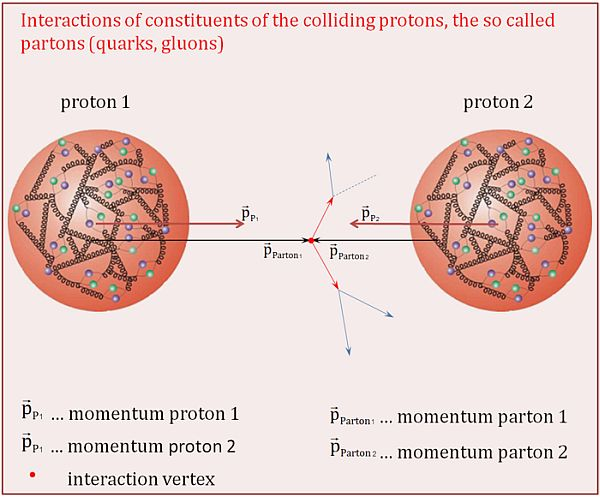
\includegraphics[scale=0.55]{proton_proton_1.png}
\caption[Proton-Proton collision]{Proton-proton collision. Protons are composed of 3 valence quarks, a sea of quarks and gluons; therefore in a proton-proton collision, quarks and gluons are those who collide. \cite{pp_coll}.}
\label{pp_collision}
\end{figure}

Protons are composed of quarks and these quarks are bound by gluons; however, what is commonly called the quark content of the proton makes reference to the valence quarks. In fact, a proton is not just a rigid entity with three balls in it all tied up with springs, but the gluons exchanged by the valence quarks tend to split spontaneously into quark-antiquark pairs or more gluons, creating \ti{sea of quarks and gluons} as represented in Figure \ref{pp_collision}.

In a proton-proton (\pp) collision, the proton's constituents, quarks and gluons, are whose collide and given that the \pp cross section depends on the momentum of the colliding particles, it is necessary to know how the proton's momentum is distributed among its constituents; the functions that describe how the momentum of the proton is distributed among its quarks and gluons, known as partons, are called \ti{parton distribution functions (PDFs)}; PDFs are determined from experimental data obtained in experiments where the internal structure of hadrons is tested, and depend on the momentum transfer $Q$ and the fraction of momentum $x$ carried by an specific parton. Figure \ref{fig:pdfs} shows the proton PDFs ($xf(x,Q^2)$) for two values of $Q$.     

\begin{figure}[!h]
\centering
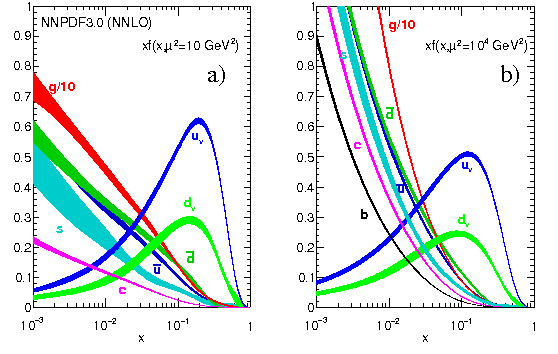
\includegraphics[width=0.8\textwidth]{pdfs_1.png}
\caption[Proton PDFs]{Proton PDFs for two values of $Q^2$: left.$\mu^2=Q^2=10$ GeV$^2$ , right. $\mu^2=Q^2=10$ GeV$^2$. $u_v$ and $d_v$ correspond to the $u$ and $d$ valence quarks, $s, c, b, \bar{u}, \bar{d}$ correspond to sea quarks, and $g$ corresponds to gluons. Note that glouns carry a high fraction of the proton's momentum \cite{pdg}.}
\label{fig:pdfs}
\end{figure}

In physics, a common approach to study complex systems consists of starting with a simpler version of them, for which a well known description is available, and adding an additional \ti{perturbation} which represents a small deviation from the known behavior. If the perturbation is small enough, the physical quantities associated with the perturbed system are expressed as a series of corrections to those of the simpler system. The perturbation series corresponds to an expansion in power series of a small parameter, therefore, the more terms are considered in the series (the higher order in the perturbation series), the more precise is the the description of the complex system. If the perturbation does not get progressively smaller, the strategy cannot be applied and new methods have to be employed. 

High energy systems, like the Higgs production at LHC explored in this thesis, usually can be treated perturbatively with the expansion made in terms of the coupling constants. The overview presented here will be oriented specifically to the Higgs boson production mechanisms in \pp collisions at LHC.

\begin{figure}[!h]
\centering
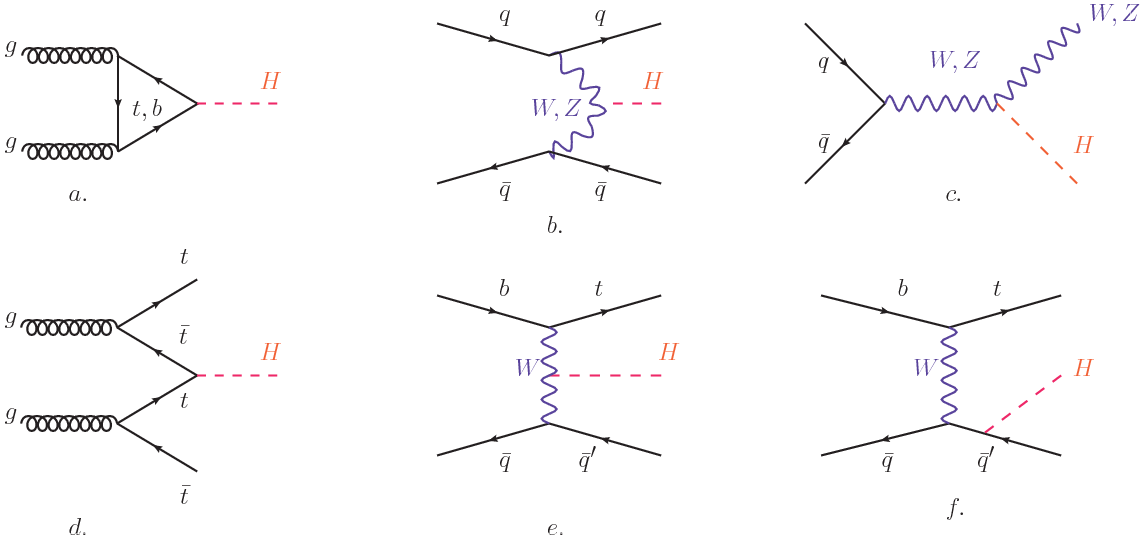
\includegraphics[width=\textwidth]{higgs_prod}
\caption[Higgs boson production mechanism Feynman diagrams]{Main Higgs boson production mechanism Feynman diagrams. a. gluon-gluon fusion, b. vector boson fusion (VBF), c. Higgs-strahlung, d. Associated production with a top or bottom quark pair, e-f. associated production with a single top quark.}
\label{higgs_prod}
\end{figure}

Figure \ref{higgs_prod} shows the Feynman diagrams for the leading order (first order LO) Higgs production processes at LHC; note that in these diagrams the incoming particles are not the protons themselves but the partons from the protons that actually participate in the interaction, hence, theorists typically calculate the cross section for the parton interaction, and then convolute that cross section with the information from the PDFs to get a production cross section that is actually measured in experiments. The cross section for Higgs production as a function of the center of mass-energy ($\sqrt{s}$) for \pp collisions is showed in Figure \ref{hcs_br} left. The tags NLO (next to leading order), NNLO (next to next to leading order) and N3LO (next to next to next to leading order) make reference to the order at which the perturbation series have been considered while the tags QCD and EW correspond to the strong and electroweak coupling constants respectively.
%% Table \ref{hxsec} present the cross sections for $m_H=125GeV/c^2$.
%% \begin{center}
%% \begin{table}[h]
%% \centering
%% \begin{tabular}{lllllll}\hline
%% $\sqrt{s}$(TeV) &\multicolumn{6}{l}{Production cross section (in pb) for $m_H$ = 125 GeV/c$^2$}\\\hline
%%                 & ggF          & VBF          & WH           & ZH           & $t\bar{t}H$           & total \\\hline
%% 7               & $16.9\pm5\%$ & $1.24\pm2\%$ & $0.58\pm3\%$ & $0.34\pm4\%$ & $0.09^{+8\%}_{-14\%}$ & 19.1  \\
%% 8               & $21.4\pm5\%$ & $1.60\pm2\%$ & $0.70\pm3\%$ & $0.42\pm5\%$ & $0.13^{+8\%}_{-13\%}$ & 24.2  \\
%% 13              & $48.6\pm5\%$ & $3.78\pm2\%$ & $1.37\pm2\%$ & $0.88\pm5\%$ & $0.50^{+9\%}_{-13\%}$ & 55.1  \\
%% 14              & $54.7\pm5\%$ & $4.28\pm2\%$ & $1.51\pm2\%$ & $0.99\pm5\%$ & $0.60^{+9\%}_{-13\%}$ & 62.1  \\\hline
%% \end{tabular}
%% \caption[The SM Higgs boson production cross sections for $m_H = 125 GeV/c^2$.]{The SM Higgs boson production cross sections for $m_H = 125 GeV/c^2$.in \pp collisions as a function of
%% the center of mass energy, $\sqrt{s}$. The predictions for the ggF channel at the LHC include the latest N3LO results leading to reduced theoretical uncertainties by a factor around 2 compared to the N2LO results.\cite{pdg}}\label{hxsec}
%% \end{table}
%% \end{center}

\begin{figure}[!h]
\centering
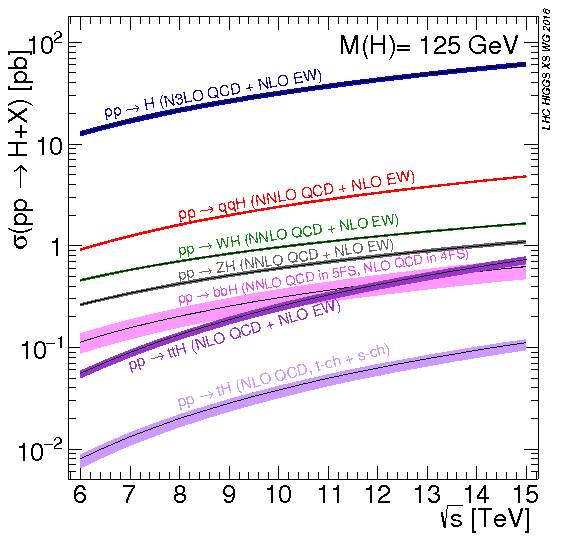
\includegraphics[width=0.45\textwidth]{higgs_prod_plot_1.png}
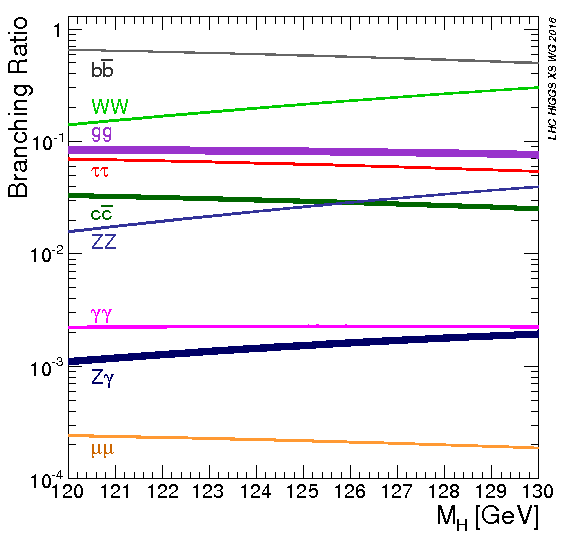
\includegraphics[width=0.45\textwidth]{higgsbr_1.png}
\caption[Higgs boson production cross section and decay branching ratios]{Higgs boson production cross sections (left) and decay branching ratios (right) for the main mechanisms. The VBF is indicated as qqH\cite{hcswg}.}
\label{hcs_br}
\end{figure}

%As shown in Eqns \ref{lyl}, \ref{lyq} and \ref{lhV}, the strength of the Higgs-fermion interaction is proportional to the fermion mass while the strength of the Higgs-gauge boson interaction is proportional to the square of the gauge boson mass, which implies that the Higgs production and decay mechanisms are dominated by couplings $H-(W,Z,t,b,\tau)$. 

The main production mechanism is the gluon fusion (Figure \ref{higgs_prod}a and $pp\to H$ in Figure \ref{hcs_br}) given that gluons carry the highest fraction of momentum of the protons in \pp colliders (as shown in Figure \ref{fig:pdfs}). Since the Higgs boson does not couple to gluons, the mechanism proceeds through the exchange of a virtual top-quark loop. Note that in this process the Higgs boson is produced alone, turning out to be problematic for some Higgs decays, because such absence of anything produced in association with the Higgs represent a trouble for triggering, however, this mechanism is experimentally clean when combined with the two-photon or the four-lepton decay channels (see Section \ref{sec:decays}). 

Vector boson fusion (Figure \ref{higgs_prod}b and $pp\to qqH$ in Figure \ref{hcs_br}) has the second largest production cross section. The scattering of two fermions is mediated by a weak gauge boson which later emits a Higgs boson. In the final state, the two fermions tend to be located in the central region of the detector; this kind of features are generally used as a signature when analyzing the datasets provided by the experiments\footnote{More details about how to identify events of interest in this analysis will be given in chapter \ref{ch:analysis}.}. 

In the Higgs-strahlung mechanism (Figure \ref{higgs_prod}c and ~$pp\to WH, pp\to ZH$ in Figure ~\ref{hcs_br}) two fermions annihilate to form a weak gauge boson. If the initial fermions have enough energy, the emergent boson might emit a Higgs boson.

The associated production with a top or bottom quark pair and the associated production with a single top quark (Figure \ref{higgs_prod}d-f and ~$pp\to bbH, pp\to \ttH, pp\to tH$ in Figure \ref{hcs_br}) have a smaller cross section than the main three mechanisms above, but they provide a good opportunity to test the Higgs-top coupling. The analysis reported in this thesis is developed using these production mechanisms. A detailed description of the \tH mechanism will be given in Section \ref{sec:thq}.  

\subsection{Higgs boson decay channels}\label{sec:decays}

When a particle can decay through several modes, also known as channels, the probability of decaying through a given channel is quantified by the \ti{branching ratio (BR)} of the decay channel; thus, the BR is defined as the ratio of number of decays going through that given channel to the total number of decays. In regard to the Higgs boson decay, the BR can be predicted with accuracy once the Higgs mass is known \cite{riley, denner}. In Figure \ref{hcs_br} right, a plot of the BR as a function of the Higgs mass is presented; the largest predicted BR corresponds to the $\bbbar$ pair decay channel (see Table \ref{hdbr}) given that it is the heaviest particle pair whose on-shell \footnote{In general, on-shell or real particles are those which satisfy the energy-momentum relation ($E^2-|\vec{p}|^2c^2= m^2c^4$); off-shell or virtual particles does not satisfy it which is possible under the uncertainty principle of quantum mechanics. Usually, virtual particles correspond to internal propagators in Feynman diagrams.} production is kinematically allowed in the decay.

\begin{table}[h]
\centering
\small
\begin{tabular}{lll}\hline
Decay channel       & Branching ratio   & Rel. uncertainty\\\hline
$H\to b\bar{b}$     & $5.84\times10^{-1}$ & $+3.2\%-3.3\%$\\
$H\to W^+W^-$       & $2.14\times10^{-1}$ & $+4.3\%-4.2\%$\\
$H\to\tau^+\tau^-$  & $6.27\times10^{-2}$ & $+5.7\%-5.7\%$\\
$H\to ZZ$           & $2.62\times10^{-2}$ & $+4.3\%-4.1\%$\\
$H\to \gamma\gamma$ & $2.27\times10^{-3}$ & $+5.0\%-4.9\%$\\
$H\to Z\gamma$      & $1.53\times10^{-3}$ & $+9.0\%-8.9\%$\\
$H\to\mu^+\mu^-$    & $2.18\times10^{-4}$ & $+6.0\%-5.9\%$\\\hline
\end{tabular}
\caption[Predicted branching ratios for a SM Higgs boson with $m_H = 125$ GeV/c$^2$.]{Predicted branching ratios and the relative uncertainty for some decay channels of a SM Higgs boson with $m_H = 125$ GeV/c$^2$ \cite{pdg}%; the uncertainties are driven by theoretical uncertainties for the different Higgs boson partial widths and by parametric uncertainties associated to the strong coupling and the masses of the quarks which are the input parameters. Further details on these calculations can be found in Reference \cite{florian}
}\label{hdbr}
\end{table}

Decays to other lepton and quark pairs, like electron, strange, up, and down quark pairs not listed in the table, are also possible but their likelihood is too small to measure since they are very lightweight, hence, their interaction with the Higgs boson is very weak. On other hand, the decay to top quark pairs is heavily suppressed due to the top quark mass ($\approx 173$ GeV/c$^2$).

Decays to gluons proceed indirectly through a virtual top quark loop while the decays to photons proceed through a virtual W boson loop, therefore, their branching ratio is smaller compared to direct interaction decays. Same is true for the decay to a photon and a Z boson.

In the case of decays to pairs of W and Z bosons, the decay proceed with one of the bosons being on-shell and the other being off-shell. The likelihood of the process diminish depending on how far off-shell are the virtual particles involved, hence, the branching ratio for W boson pairs is bigger than for Z boson pairs since Z boson mass is bigger than W boson mass.

Note that the decay to a pair of virtual top quarks is possible, but the probability is way too small. 

\section{Experimental status of the anomalous Higgs-fermion coupling}

\begin{figure}[h!]
\centering
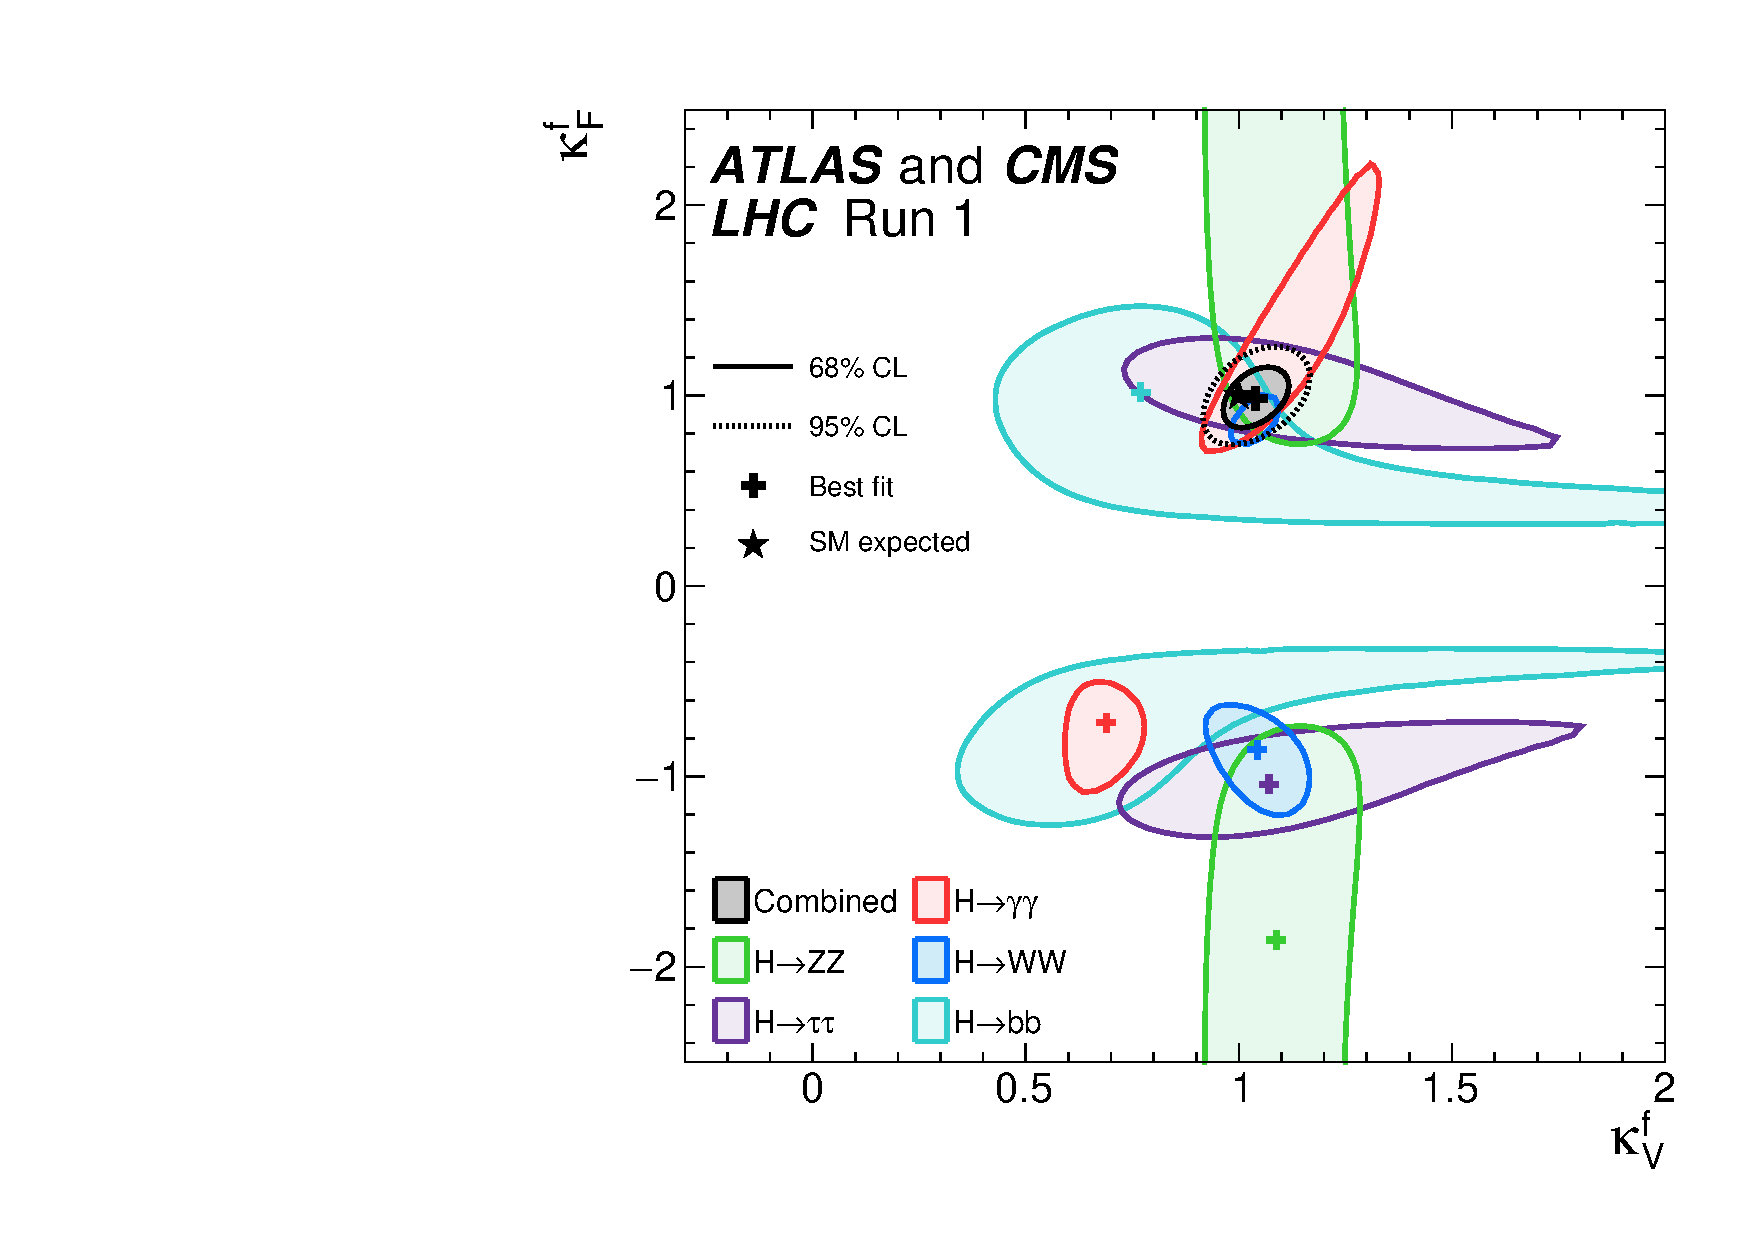
\includegraphics[scale=0.5]{kt_kv}
\caption[$\kappa_t$-$\kappa_V$ plot of the coupling modifiers. ATLAS and CMS combination.]{Combination of the  ATLAS and CMS fits for coupling modifiers $\kappa_t$-$\kappa_V$; also shown the individual decay channels combination and their global combination. No assumptions have been made on the sign of the coupling modifiers\cite{comb_ht_couplings}.} 
\label{fig:kt_kv}
\end{figure}
 
ATLAS and CMS have performed analyses of the anomalous Higgs-fermion coupling by making likelihood scans for the two coupling modifiers, $\kappa_f$ and $\kappa_V$, under the assumption that $\kappa_Z=\kappa_W \equiv \kappa_V$ and $\kappa_t=\kappa_\tau=\kappa_b \equiv\kappa_f$. Figure \ref{fig:kt_kv} shows the result of the combination of ATLAS and CMS fits; also the individual decay channels combination and the global combination results are shown. Note that from this plot there is limited information on the sign of the coupling since the only information available about the sign of the coupling comes from decays rather than production. 

While all the channels are compatible for positive values of the modifiers, for negative values of $\kappa_f$ there is no compatibility. The best fit for individual channels is compatible with negative values of $\kappa_f$ except for the $H\to bb$ channel. The best fit for the combination yields $\kappa_f\geq0$, in contrast to the yields from the individual channels; the reason of this yield resides in the H $\to \gamma \gamma$ coupling. H $\to \gamma \gamma$ decay proceeds through a loop of either top quarks or W bosons, hence, this channel is sensitive to \Ct thanks to the interference of these two amplitude contributions; under the assumption that no beyond SM particles take part in the loops, a flipped sign of \Ct will increase the H $\to \gamma \gamma$ branching fraction by a factor of $\sim$ 2.4 which is not supported by measurements; thus, this large asymmetry between the positive and negative coupling ratios in the H $\to \gamma \gamma$ channel drives the yield of the global fit and would means that the anomalous H-t coupling is excluded as stated in Reference \cite{comb_ht_couplings}, but there is a caveat, this exclusion holds only if no new particles contribute to the loop in the main diagram for that decay.

Although the $H\to bb$ channel is expected to be the most sensitive channel and its best fit value of \Ct is positive, and then the global fit yield is still supported, the contributions from all the other decay channels, small compared to the $H\to bb$, indicate that the anomalous H-t coupling cannot be excluded completely, motivating to look at \tH processes which can help with both, the limited information on the sign of the H-t coupling and the access to information from the Higgs boson production rather that from its decays. It will be shown in Section \ref{sec:thq} that the same interference effect enhance the \tH production rate and could reveal evidence of direct production of heavy new particles as predicted in composite and little Higgs models \cite{lhiggs}, or new physics related to Higgs boson mediated flavor changing neutral currents \cite{greljo} as well as probes the CP-violating phase of the H-t coupling \cite{maltoni2, demartin}.

%______________________ tHq ______________________
\section{Associated production of a Higgs boson and a single top quark}\label{sec:thq}

\begin{figure}[h!]
\centering
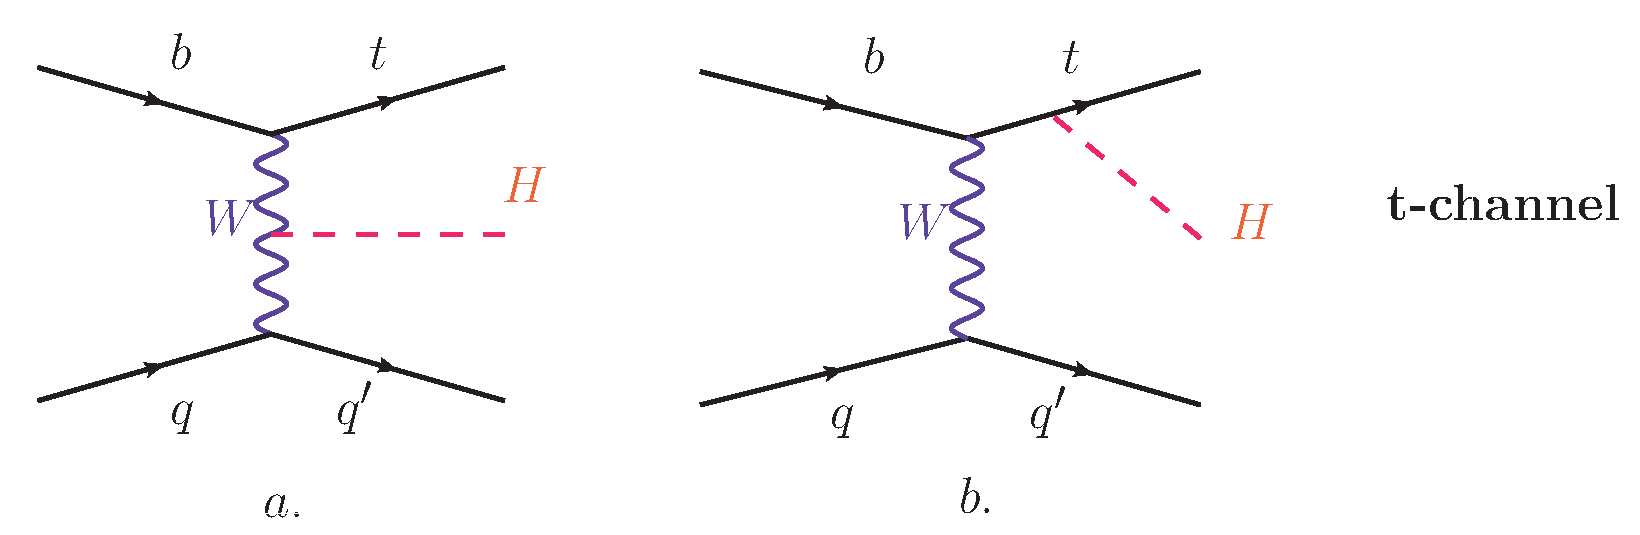
\includegraphics[scale=0.4]{thq_prod}\\
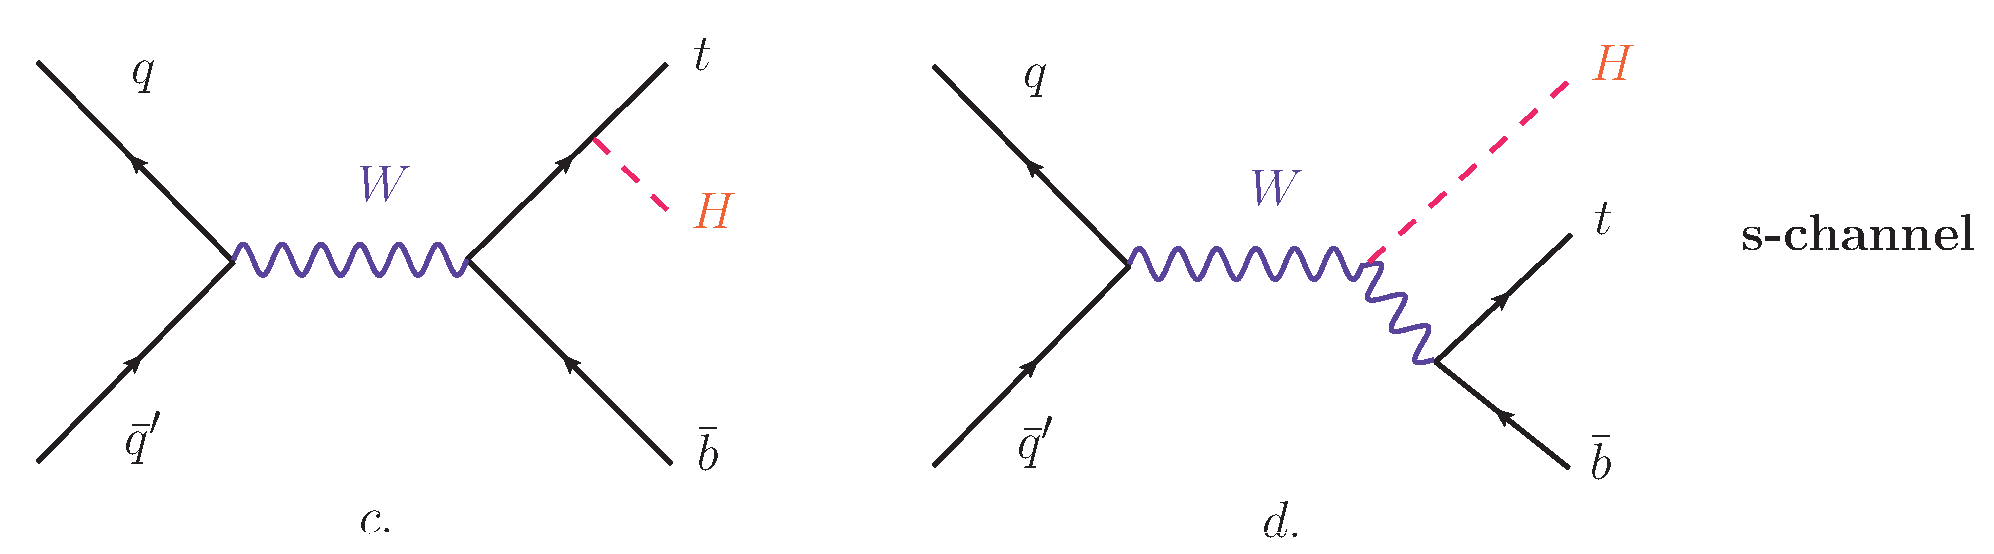
\includegraphics[scale=0.4]{thb_prod}\\
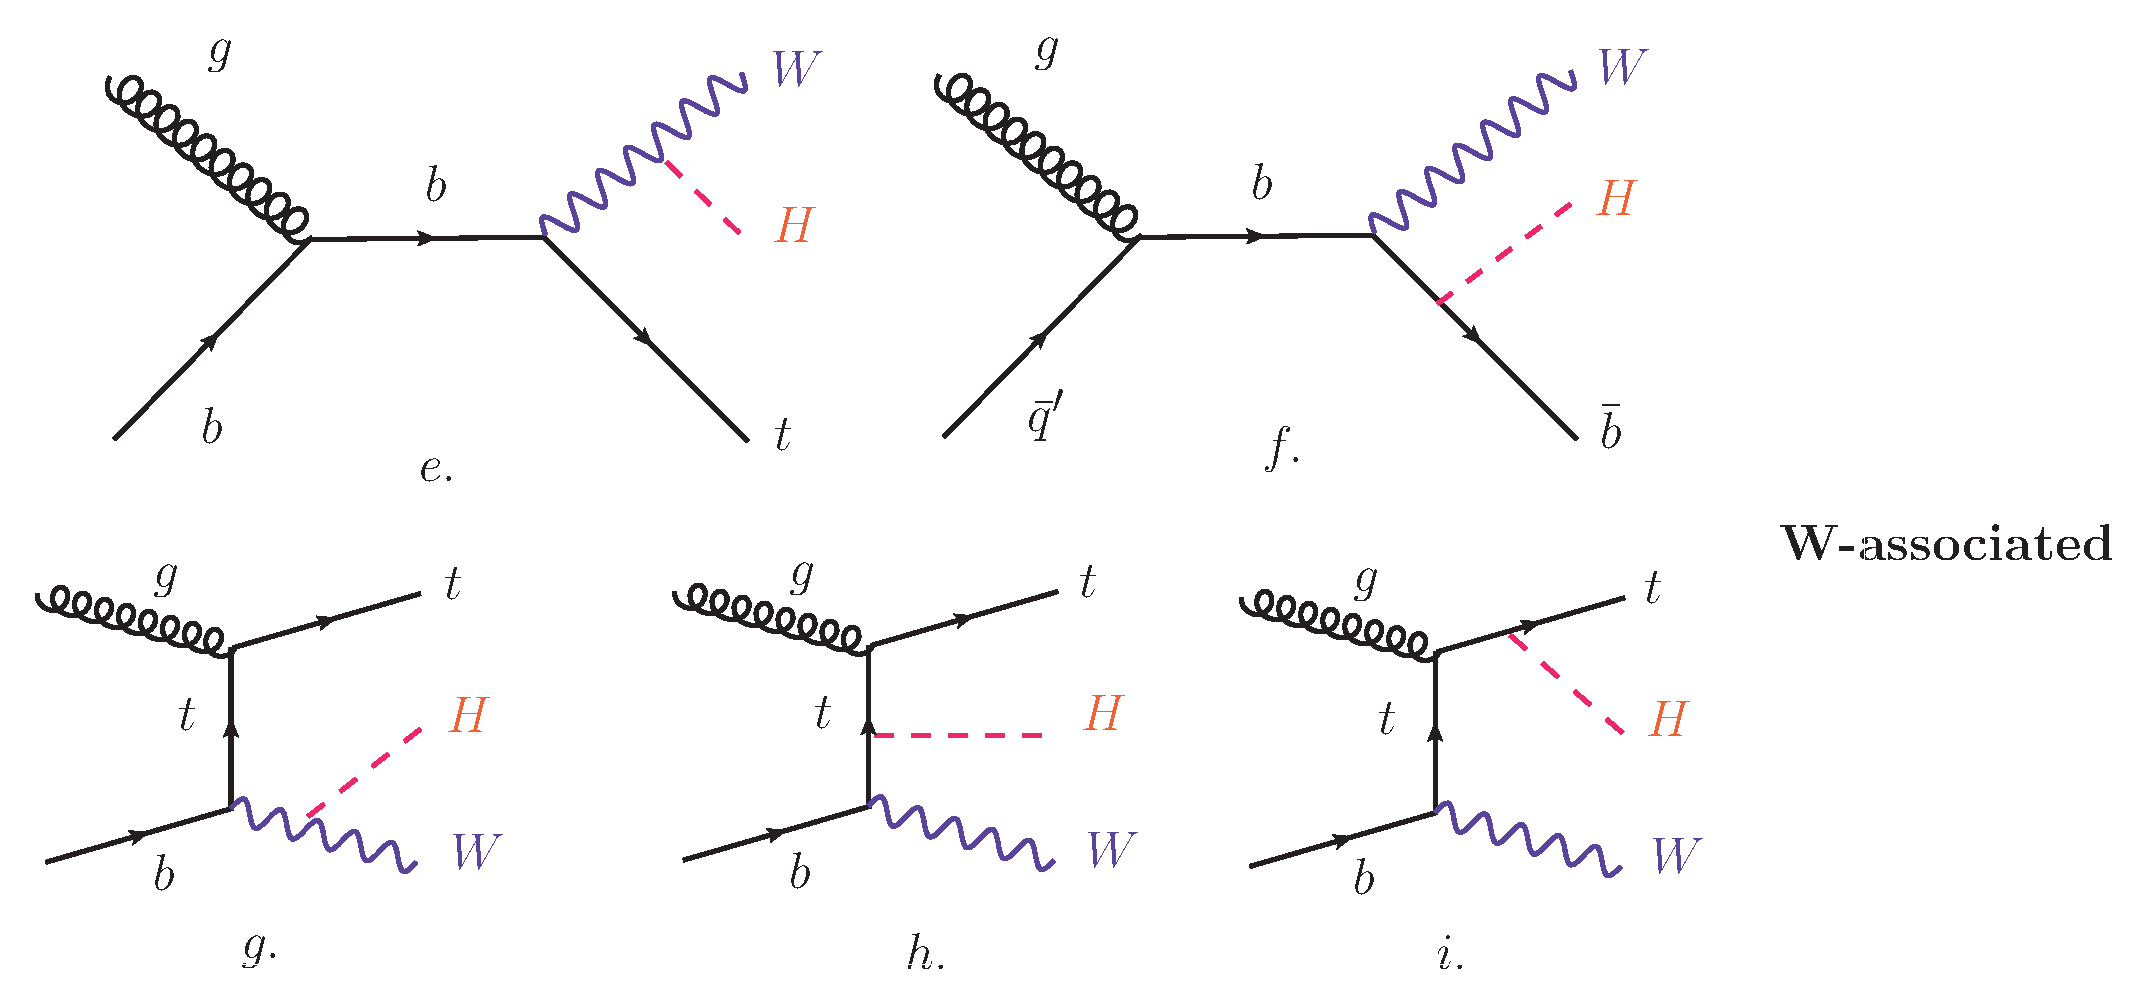
\includegraphics[scale=0.4]{thW_prod}\\
\caption[Higgs boson production in association with a top quark]{Associated Higgs boson production with a top quark mechanism Feynman diagrams. a.,b. t-channel (\tHq), c.,d. s-channel ($tHb$), e-i. W-associated.}
\label{fig:th_prod}
\end{figure}

The production of Higgs boson in association with a top quark has been extensively studied \cite{maltoni1, biswas, farina,tait, maltoni2}. While measurements of the main Higgs production mechanisms rates are sensitive to the strength of the Higgs coupling to W boson or top quark, they are not sensitive to the relative sign between the two couplings. In this thesis, the Higgs boson production mechanism explored is the associated production with a single top quark (\tH) which offers sensitivity to the relative sign of the Higgs couplings to W boson and to top quark. The description given here is based on Reference \cite{farina}.

A process where two incoming particles interact and produce a final state with two particles can proceed in three called channels (see, for instance, Figure \ref{fig:th_prod} omitting the red line). The t-channel represents processes where an intermediate particle is emitted by one of the incoming particles and absorbed by the other. The s-channel represents processes where the two incoming particles merge into an intermediate particle which eventually will split into the particles in the final state. The third channel, u-channel, is similar to the t-channel but the two outgoing particles interchange their roles. These three channels are connected to the so-called Mandelstam variables 

\begin{align}
&s =(p_1 +p_2)^2 =(p_1' + p_2')^2 \to{\small \textrm{ square of the center mass-energy}}.\\
&t =(p_1 -p_1')^2 =(p_2' -p_2)^2 \to{\small \textrm{ square of the four-momentum transfer}}.\\
&u =(p_1 -p_2')^2 =(p_1' - p_2)^2 \to{\small \textrm{ square of the crossed four-momentum transfer}}.\\
&s+t+u = m_1^2 + m_2^2 + m_1^{'2} +  m_2^{'2}
\end{align}

\noindent which relate the momentum, energy and the angles of the incoming and outgoing particles in an scattering process of two particles to two particles. The importance of the Mandelstam variables reside in that they form a minimum set of variables needed to describe the kinematics of this scattering process; they are Lorentz invariant which makes them very useful when doing calculations.      

The \tH production, where Higgs boson can be radiated either from the top quark or from the W boson, is represented by the leading order Feynman diagrams in Figure \ref{fig:th_prod}. The cross section for the \tH process is calculated, as usual, summing over the contributions from the different Feynman diagrams; therefore it depends on the interference between the contributions. In the SM, the interference for t-channel (\tHq process)  and W-associated (\tHW process) production is destructive \cite{maltoni1} resulting in the small cross sections presented in Table \ref{tab:th_xsec}. 

\begin{table}[h]
\centering
\begin{tabular}{lll}\hline
tH production channel       & Cross section (fb)      \\\hline
t-channel $(pp \to tHq)$    & $70.79^{+2.99}_{-4.80}$ \\
W-associated $(pp \to tHW)$ & $15.61^{+0.83}_{-1.04}$ \\
s-channel$(pp \to tHb)$     & $ 2.87^{+0.09}_{-0.08}$ \\\hline
\end{tabular}
\caption[Predicted SM cross sections for \tH production at $\sqrt{s}=13$ TeV.]{Predicted SM cross sections for \tH production at $\sqrt{s}=13$ TeV \cite{thqw_xsec, thb_xsec}.}\label{tab:th_xsec}
\end{table}

The s-channel contribution can be neglected. It will be shown that a deviation from the SM destructive interference would result in an enhancement of the \tH cross section compared to that in SM, which could be used to get information about the sign of the Higgs-top coupling \cite{farina,tait}. In order to describe \tH production processes, Feynman diagram \ref{fig:th_prod}b will be considered; there, the W boson is radiated by a quark in the proton and eventually it will interact with the b quark. In the high energy regime, the effective W approximation \cite{dawson} is used to describe the process as the emission of an approximately on-shell W and its hard scattering with the b quark; \ie $Wb \to th$. The scattering amplitude for the process is given by

\begin{equation} \label{s_amp}
\begin{split}
\mathcal{A}= &\frac{g}{\sqrt{2}}(\kappa_t-\kappa_V)\frac{m_t\sqrt{s}}{m_Wv} A\left(\frac{t}{s},\varphi; \xi_{t},\xi_{b}\right) +\\ & \frac{g}{\sqrt{2}} \left(\kappa_V\,\frac{2m_W}{v}\frac{s}{t}+(2\kappa_t-\kappa_V)\,\frac{m_t^{2}}{m_Wv}\right)\,B\left(\frac{t}{s},\varphi; \xi_{t},\xi_{b}\right),
\end{split}
\end{equation}

\noindent where $\kappa_V\equiv g_{HVV}/g_{HVV}^{SM}$ and $\kappa_t\equiv g_{Ht}/g_{Ht}^{SM}=y_t/y_t^{SM}$ are scaling factors that quantify possible deviations of the couplings from the SM values, Higgs-Vector boson (H-W) and Higgs-top (H-t) respectively, from the SM couplings; ${s=(p_{W}+p_{b})^{2}}$, ${t=(p_{W}-p_{H})^{2}}$, $\varphi$ is the Higgs azimuthal angle around the $z$ axis taken parallel to the direction of motion of the incoming W; A and B are functions describing the weak interaction in terms of the chiral states ($\xi_{t},\xi_{b}$) of the quarks $b$ and $t$.

Terms that vanish in the high energy limit have been neglected as well as the Higgs and \textit{b} quark masses\footnote{A detailed explanation of the structure and approximations used to derive $\mathcal{A}$ can be found in Reference \cite{farina}}.

The scattering amplitude grows with energy like $\sqrt{s}$ for $\kappa_V \neq \kappa_t$ , in contrast to the SM ($\kappa_t=\kappa_V=1$), where the first term in \ref{s_amp} cancels out and the amplitude is constant for large s; therefore, a deviation from the SM predictions represents an enhancement in the \tHq cross section. In particular, for a SM H-W coupling and a H-t coupling of inverted sign with respect to the SM ($\kappa_V =-\kappa_t=1$) the \tHq cross section is enhanced by a factor greater 10 as seen in the Figure \ref{thq_en} taken from Reference \cite{farina}; Reference \cite{biswas2} has reported similar enhancement results.

\begin{figure}[h!]
\centering
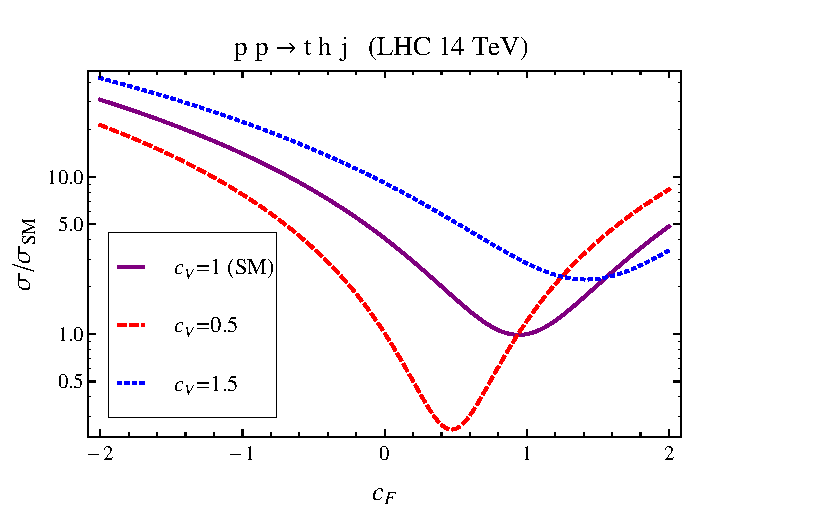
\includegraphics[scale=0.9]{thq_en}
\caption[Cross section for \tHq process as a function of $\kappa_t$]{Cross section for \tHq process as a function of $\kappa_t$, normalized to the SM, for three values of $\kappa_V$. In the plot $c_f$ refers to the Higgs-fermion coupling which is dominated by the H-t coupling and represented in this analysis by \Ct; $c_{V}$ refers to the Higgs-vector boson (W/Z) coupling represented in this analysis by \CV. Solid, dashed and dotted lines correspond to $c_V \to \kappa_V= 1, 0.5, 1.5$ respectively. Note that for the SM scenario (${\CV=\Ct=1}$), the destructive effect of the interference is maximal.} 
\label{thq_en}
\end{figure}

\begin{figure}[h!]
\centering
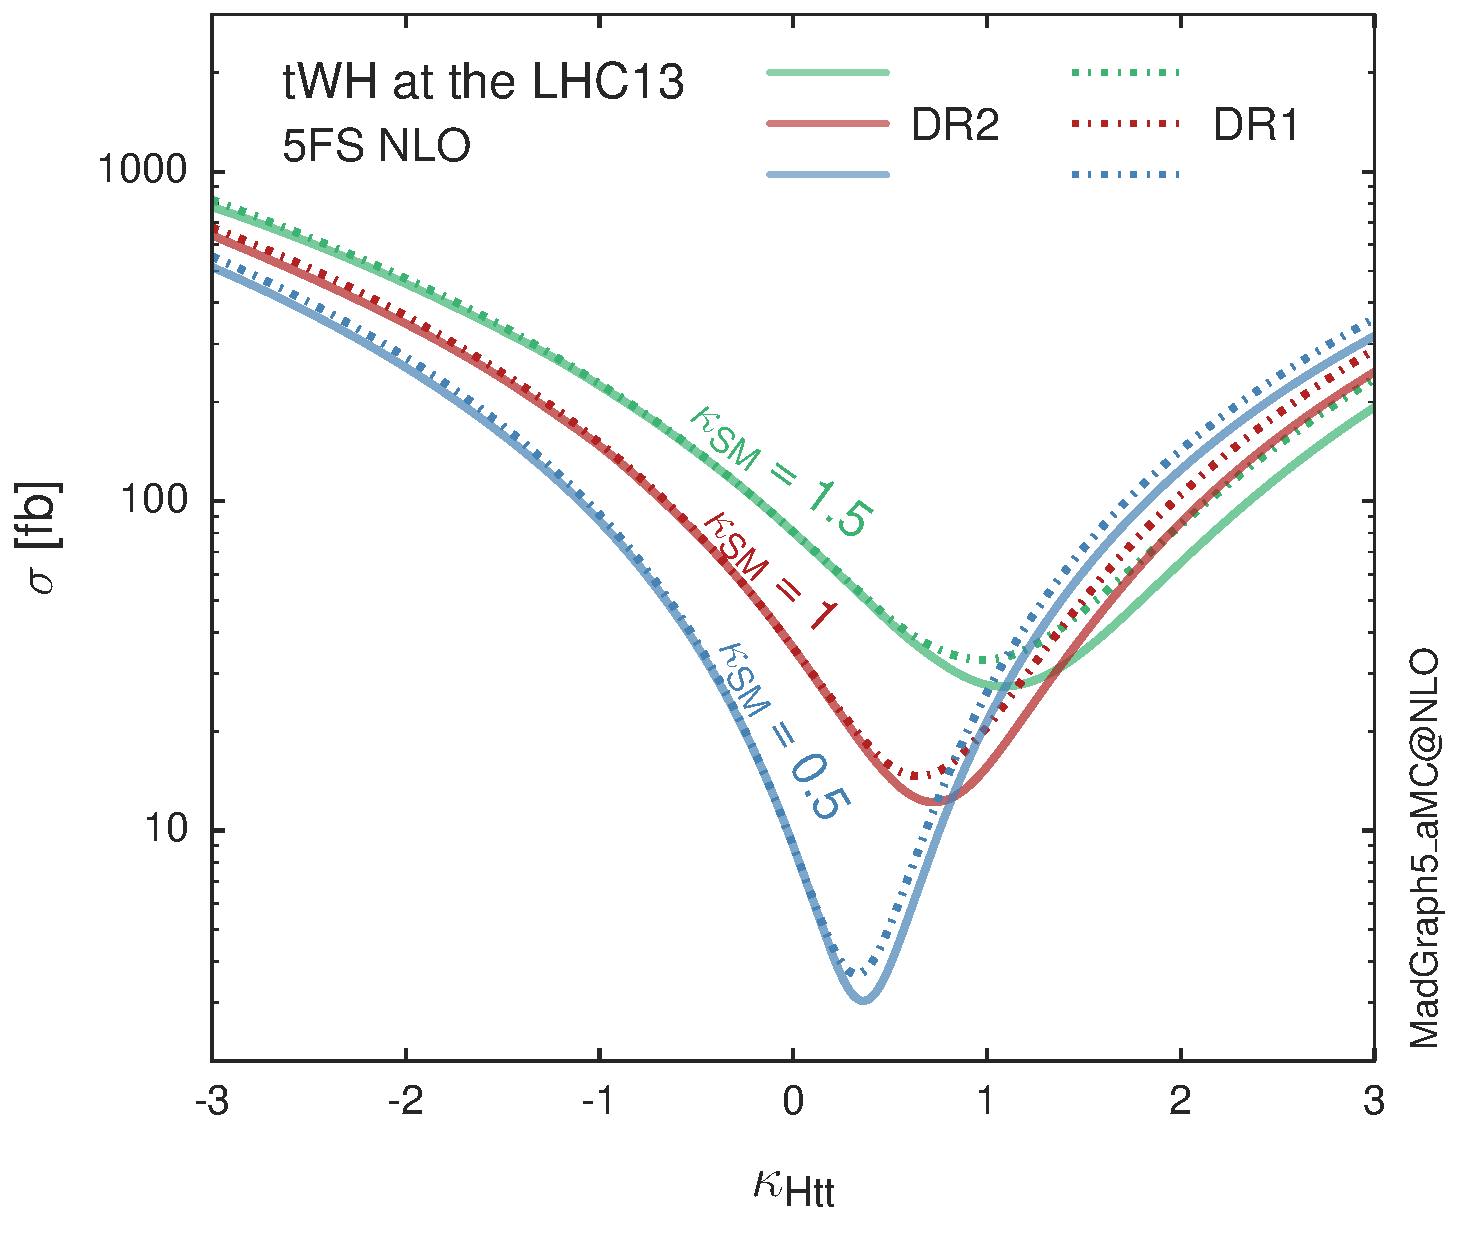
\includegraphics[scale=0.4]{thw_en}
\caption[Cross section for \tHW process as a function of $\kappa_{Htt}$]{Cross section for \tHW process as a function of $\kappa_{Htt}$, for three values of $\kappa_{SM}$ at $\sqrt{s}=13$ TeV. $\kappa_{Htt}^2=\sigma_{Htt}/\sigma_{Htt}^{SM}$ is a simple re-scaling of the SM Higgs interactions.} 
\label{thw_en}
\end{figure}

A similar analysis is valid for the W-associated channel but, in that case, the interference is more complicated since there are more than two contributions and an additional interference with the production of Higgs boson and a top pair process(\ttH). The calculations are made using the so-called Diagram Removal (DR) technique where interfering diagrams are removed (or added) from the calculations in order to evaluate the impact of the removed contributions. DR1 was defined to neglect \ttH interference while DR2 was defined to take \ttH interference into account\cite{demartin}. As shown in Figure \ref{thw_en}, the \tHW cross section is enhanced from about 15 fb (SM: $\kappa_{Htt}=1$) to about 150 fb ($\kappa_{Htt}=-1$). Differences between curves for DR1 and DR2 help to gauge the impact of the interference with \ttH.     
Results of the calculations of the \tHq and \tHW cross sections at $\sqrt{s}=13$ TeV can be found in Reference \cite{yellow} and a summary of the results is presented in Table \ref{tab:th_xsec_en}.

\begin{table}[h]
\centering
\begin{tabular}{lcll}\hline
                                                            & $\sqrt{s}$ TeV   & $\kappa_t=1$                        & $\kappa_t=-1$                   \\\hline
\multirow{2}{*}{$\sigma^{LO}$(\tHq)(fb)\cite{farina}}       & 8                & $\approx 17.4$                 & $\approx 252.7$            \\
                                                            & 14               & $\approx 80.4$                 & $\approx 1042$             \\\hline
\multirow{2}{*}{$\sigma^{NLO}$(\tHq)(fb)\cite{farina}}      & 8                & $18.28^{+0.42}_{-0.38}$        & $233.8^{+4.6}_{-0.0}$      \\
                                                            & 14               & $88.2^{+1.7}_{-0.0}$           & $982.8^{+28}_{-0.0}$       \\\hline
$\sigma^{LO}$(\tHq)(fb) \cite{biswas2}                      & 14               & $\approx 71.8$                 & $\approx 893$              \\
$\sigma^{LO}$(\tHW)(fb) \cite{biswas2}                      & 14               & $\approx 16.0$                 & $\approx 139$              \\\hline
\multirow{3}{*}{$\sigma^{NLO}$(\tHq)(fb)\cite{yellow}}      & 8                & $18.69^{+8.62\%}_{-17.13\%}$   & -                          \\
                                                            & 13               & $74.25^{+7.48\%}_{-15.35\%}$   & $848^{+7.37\%}_{-13.70\%}$ \\
                                                            & 14               & $90.10^{+7.34\%}_{-15.13\%}$   & $1011^{+7.24\%}_{-13.39\%}$\\\hline
$\sigma^{LO}$(\tHW)(fb)\cite{demartin}                      & 13               & $15.77^{+15.91\%}_{-15.76\%}$  & -                          \\
$\sigma^{NLO} DR1$(\tHW)(fb)\cite{demartin}                 & 13               & $21.72^{+6.52\%}_{-5.24\%}$    & $\approx 150$              \\
$\sigma^{NLO} DR2$(\tHW)(fb)\cite{demartin}                 & 13               & $16.28^{+7.34\%}_{-15.13\%}$   & $\approx 150$              \\\hline
\end{tabular}
\caption[Predicted enhancement of the \tHq and \tHW cross sections at LHC]{Predicted enhancement of the \tHq and \tHW cross sections at LHC for $\kappa_V=1$ and $\kappa_t= \pm1$ at LO and NLO; the cross section enhancement of more that a factor of 10 is due to the flipping in the sign of the H-t coupling with respect to the SM one.}
\label{tab:th_xsec_en}
\end{table}

%% \begin{center}
%% \begin{table}[h]
%% \centering
%% \begin{tabular}{lcll}\hline
%%                                                             & $\sqrt{s}$ TeV   & $\kappa_t=1$                        & $\kappa_t=-1$                   \\\hline
%% \multirow{2}{*}{$\sigma^{LO}$(\tHq)(fb)\cite{farina}}       & 8                & $\approx 17.4$                 & $\approx 252.7$            \\
%%                                                             & 14               & $\approx 80.4$                 & $\approx 1042$             \\\hdashline
%% $\sigma^{LO}$(\tHq)(fb) \cite{biswas2}                      & 14               & $\approx 71.8$                 & $\approx 893$              \\
%% $\sigma^{LO}$(\tHW)(fb) \cite{biswas2}                      & 14               & $\approx 16.0$                 & $\approx 139$              \\%\hline
%% $\sigma^{LO}$(\tHW)(fb)\cite{demartin}                      & 13               & $15.77^{+15.91\%}_{-15.76\%}$  & -                          \\\hline
%% \multirow{2}{*}{$\sigma^{NLO}$(\tHq)(fb)\cite{farina}}      & 8                & $18.28^{+0.42}_{-0.38}$        & $233.8^{+4.6}_{-0.0}$      \\
%%                                                             & 14               & $88.2^{+1.7}_{-0.0}$           & $982.8^{+28}_{-0.0}$       \\\hdashline
%% \multirow{3}{*}{$\sigma^{NLO}$(\tHq)(fb)\cite{yellow}}      & 8                & $18.69^{+8.62\%}_{-17.13\%}$   & -                          \\
%%                                                             & 13               & $74.25^{+7.48\%}_{-15.35\%}$   & $848^{+7.37\%}_{-13.70\%}$ \\
%%                                                             & 14               & $90.10^{+7.34\%}_{-15.13\%}$   & $1011^{+7.24\%}_{-13.39\%}$\\\hdashline
%% $\sigma^{NLO} DR1$(\tHW)(fb)\cite{demartin}                 & 13               & $21.72^{+6.52\%}_{-5.24\%}$    & $\approx 150$              \\
%% $\sigma^{NLO} DR2$(\tHW)(fb)\cite{demartin}                 & 13               & $16.28^{+7.34\%}_{-15.13\%}$   & $\approx 150$              \\\hline
%% \end{tabular}
%% \caption[Predicted enhancement of the \tHq and \tHW cross sections at LHC]{Predicted enhancement of the \tHq and \tHW cross sections at LHC for $\kappa_V=1$ and $\kappa_t= \pm1$ at LO and NLO; the cross section enhancement of more that a factor of 10 is due to the flippling in the sign of the H-t coupling with respect to the SM one.}
%% \label{tab:th_xsec_en}
%% \end{table}
%% \end{center}

%______________________ cp phase ______________________
\section{CP-mixing in \tH processes}\label{sec:cp}

In addition to the sensitivity to sign of the H-t coupling, the \tHq and \tHW\ processes have been proposed as a tool to investigate the possibility of a H-t coupling that does not conserve CP\cite{maltoni2,demartin,ellis}. %Current experimental results are consistent with SM H-V and H-t couplings; however, negative H-t coupling is not excluded completely \cite{comb_ht_couplings}.\\

In this thesis, the sensitivity of \tH\ processes to CP-mixing is also studied on the basis of References \cite{maltoni2,demartin} using the effective field theory framework where a generic particle ($X_0$) of spin-0 and a general CP violating interaction with the top quark (Htt coupling), can couple to scalar and pseudo-scalar fermionic densities. The H-W interaction is assumed to be SM-like. The Lagrangian modeling the H-t interaction is given by

\beqn
\Lagr_0^t = -\bar\psi_t\left(c_{\alpha}\kappa_{Htt}g_{Htt}+i s_{\alpha}\kappa_{Att}g_{Att}\gamma_5 \right)\psi_t X_0,
\label{eq:l_cp}
\eeqn

\noindent where $\alpha$ is the CP-mixing phase, $c_\alpha\equiv\cos\alpha$ and $s_\alpha\equiv\sin\alpha$, $\kappa_{Htt}$ and $\kappa_{Att}$ are real dimensionless re-scaling parameters\footnote{analog to $\kappa_t$ and $\kappa_V$} used to parametrize the magnitude of the CP-violating and CP-conserving parts of the amplitude. The model defines $g_{Htt}=g_{Att}=m_t/v=y_t/\sqrt{2}$ with $v\sim 246$ GeV the Higgs vacuum expectation value. In this parametrization, three special cases can be recovered

\begin{itemize}
\item CP-even coupling $\to \alpha=0^o$  
\item CP-odd coupling $\to \alpha=90^o$
\item SM coupling $\to \alpha=0^o$ and $\kappa_{Htt}=1$  
\end{itemize}

The loop induced $X_0$ coupling to gluons can also be described in terms of the parametrization above, according to

\beqn
\Lagr_0^{g} = -\frac{1}{4}\left(c_{\alpha}\kappa_{Hgg}g_{Hgg}G_{\mu\nu}^aG^{a,\mu\nu}+s_{\alpha}\kappa_{Agg}g_{Agg}G_{\mu\nu}^a\widetilde G^{a,\mu\nu} \right)X_0.
\label{eq:l_Hglu}
\eeqn

\noindent where $g_{Hgg}=-\alpha_s/3\pi v$ and $g_{Agg}= \alpha_s/2\pi v$ and $G_{\mu\nu}$ is the gluon field strength tensors. Under the assumption that the top quark dominates the gluon-fusion process at LHC energies, $\kappa_{Hgg} \to \kappa_{Htt}$ and  $\kappa_{Agg} \to \kappa_{Att}$, so that the ratio between the gluon-gluon fusion cross section for $X_0$ and for the SM Higgs prediction can be written as     

\beqn
\frac{\sigma_{NLO}^{gg \to X_0} }{\sigma_{NLO,SM}^{gg \to H}}=  c^2_\alpha\kappa^2_{Htt}+s^2_\alpha \left( \kappa_{Att}\frac{g_{ Agg}}{g_{Hgg}} \right)^2.
\label{eq:GFrate}
\eeqn

If the re-scaling parameters are set to

\beqn
\kappa_{Htt}=1, \qquad \kappa_{Att}= \left|\frac{g_{Hgg}}{g_{Agg}}\right|=\frac{2}{3}.
\eeqn

\noindent the gluon-fusion SM cross section is reproduced for every value of the CP-mixing angle $\alpha$; therefore, by imposing that condition to the Lagrangian density \ref{eq:l_cp}, the CP-mixing angle is not constrained by current data. Figure \ref{xsec_alpha_thq} shows the NLO cross sections for t-channel $tX_0$(blue) and $t\bar{t}X_0$ (red) associated production processes as a function of the CP-mixing angle $\alpha$. $X_0$ is a generic spin-0 particle with top quark CP-violating coupling. Re-scaling factors $\kappa_{Htt}$ and  $\kappa_{Att}$ have been set to reproduce the SM gluon-fusion cross sections.   

\begin{figure}[h!]
\centering
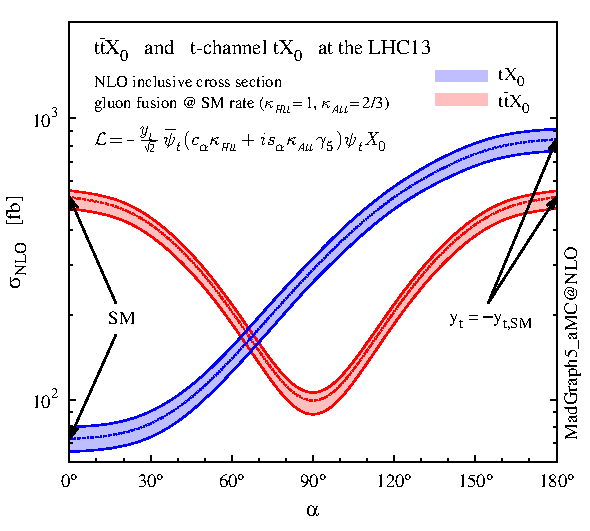
\includegraphics[scale=1.2]{xsec_alpha_thq}
\caption[NLO cross section for $tX_0$ and $t\bar{t}X_0$.]{NLO cross sections for t-channel $tX_0$(blue) and $t\bar{t}X_0$ (red) associated production processes as a function of the CP-mixing angle $\alpha$. $X_0$ is a generic spin-0 particle with top quark CP-violating coupling \cite{maltoni2}.} 
\label{xsec_alpha_thq}
\end{figure}

It is interesting to notice that the $tX_0$ cross section is enhanced, by a factor of about 10, when a continuous rotation in the scalar-pseudoscalar plane is applied; this enhancement is similar to the enhancement produced when the H-t coupling is flipped in sign with respect to the SM ($y_t=-y_{t,SM}$ in the plot), as showed in Section \ref{sec:thq}. In contrast, the degeneracy in the $t\bar{t}X_0$ cross section is still present given that it depends quadratically on the H-t coupling, but more interesting is to notice that $t\bar{t}X_0$ cross section is exceeded by $tX_0$ cross section after $\alpha\sim 60^o$.
\begin{figure}[h!]
\centering
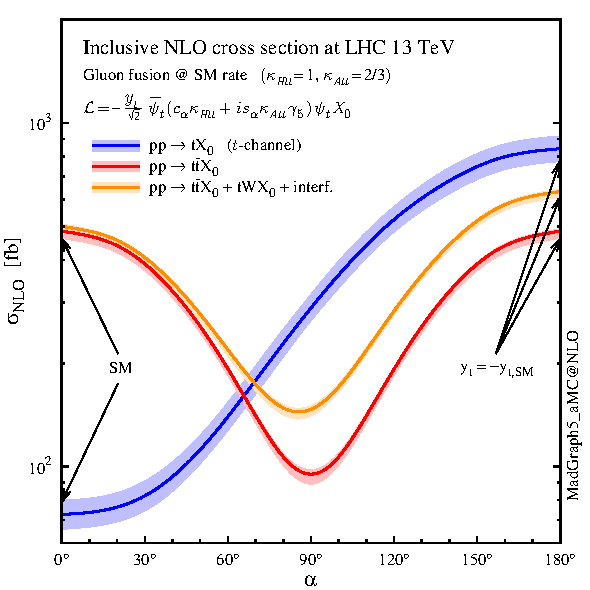
\includegraphics[scale=1.1]{xsec_alpha_thw}
\caption[NLO cross section for $tWX_0$, $t\bar{t}X_0$.]{NLO cross sections for t-channel $tX_0$(blue), $t\bar{t}X_0$ (red) associated production processes and combined $tWX_0 + t\bar{t}X_0$ (including interference) production as a function of the CP-mixing angle $\alpha$\cite{maltoni2}.} 
\label{xsec_alpha_thw}
\end{figure}

A similar parametrization can be used to investigate the \tHW process sensitivity to CP-violating H-t coupling. As said in \ref{sec:thq}, the interference in the W-associated channel is more complicated because there are more than two contributions and also there is interference with the \ttH production process.

Figure \ref{xsec_alpha_thw} shows the NLO cross sections for t-channel $tX_0$(blue), $t\bar{t}X_0$ (red) associated production and for the combined  $tWX_0 + t\bar{t}X_0 + interference$ (orange) as a function of the CP-mixing angle. It is clear that the effect of the interference in the combined case is the lifting of the degeneracy present in the $t\bar{t}X_0$ production. The constructive interference enhances the cross section from about 500 fb at SM ($\alpha=0$) to about 600 fb ($\alpha=180^o \to y_t=-y_{t,SM}$).  

An analysis combining \tHq and \tHW processes will be made in this thesis taking advantage of the sensitivity improvement.

